\documentclass[12pt,a4paper]{scrartcl}
\usepackage{amsmath}
\usepackage{amsfonts}
\usepackage[latin1]{inputenc}
\usepackage{mathptmx}
\usepackage{amscd}
\usepackage{array}
\usepackage{color}
\usepackage{hyperref}
\usepackage{url}
\usepackage{graphicx}

\usepackage{booktabs}

%\textwidth=15cm \textheight=22cm \topmargin=0.5cm
%\oddsidemargin=0.5cm \evensidemargin=0.5cm

\usepackage[T1]{fontenc}

\usepackage[scaled=0.8]{beramono}

\usepackage{fancyvrb}
\RecustomVerbatimEnvironment{Verbatim}{Verbatim}%
{xleftmargin=15pt}


\newcounter{listi}
\newcommand{\stdli}{ \topsep0ex \partopsep0ex % .5ex plus.25ex minus.125ex%
    \parsep.2ex plus.1ex minus.1ex \itemsep0ex% .5ex plus.25ex minus.125ex%
    \leftmargin2.5em \labelwidth2em \labelsep.5em \rightmargin0em}% \samepage }
\newenvironment{arab}{\begin{list}{\textup{(\arabic{listi})}}%
    {\usecounter{listi}\stdli}}{\end{list}}
\newenvironment{rome}{\begin{list}{\textup{(\roman{listi})}}%
    {\usecounter{listi}\stdli}}{\end{list}}
\newenvironment{latin}{\begin{list}{\textup{(\alph{listi})}}%
    {\usecounter{listi}\stdli}}{\end{list}}
\renewenvironment{itemize}{\begin{list}{{$\bullet$}}{\stdli}}{\end{list}}
\newenvironment{myverb}{\begin{small}}{\end{small}\pagebreak[2]}  %%%%%  \vspace{-0.8\baselineskip}




\let\phi=\varphi

\def\CC{{\mathbb C}}
\def\ZZ{{\mathbb Z}}
\def\QQ{{\mathbb Q}}
\def\RR{{\mathbb R}}
\def\EE{{\mathbb E}}
\def\AA{{\mathbb A}}
\def\PP{{\mathbb P}}
\def\NN{{\mathbb N}}

\def\Ker{\operatorname{Ker}}
\def\Im{\operatorname{Im}}
\DeclareMathOperator{\gp}{gp}
\DeclareMathOperator{\rank}{rank}


\def\cG{{\mathcal G}}
\def\cR{{\mathcal R}}

\let\hat=\widehat
\let\tilde=\widetilde
\let\Bar=\overline

\let\iso=\cong

\let\epsilon=\varepsilon
\def\discuss#1{\marginparsep=1em\marginparwidth=60pt
     \marginpar{\tt \footnotesize \raggedright #1}}

\definecolor{darkgray}{gray}{0.00}

\addtokomafont{section}{\color{darkgray}}

\setkomafont{sectionentry}{\large}

\addtokomafont{subsection}{\color{darkgray}}

\addtokomafont{subsubsection}{\normalsize}

\parindent=0pt \parskip=4pt

\setcounter{tocdepth}{3}

\def\Normaliz#1+{\textsf{Normaliz}}
\def\jNormaliz#1+{\textsf{jNormaliz}}
\def\NmzIntegrate#1+{\textsf{NmzIntegrate}}

\def\itemtt[#1]{\item[\ttt{#1}]}

\def\ttt{\texttt}


\begin{document}
\vspace*{2cm}

 \centerline{\Large\bf Normaliz 2.10\footnote{The versions 2.9 and 2.10 are identical from the user view point.}} \vspace*{1cm}


\begin{center}Winfried Bruns, Bogdan Ichim and Christof
S�ger\\[14pt] \tt
wbruns@uos.de\\
bogdan.ichim@imar.ro\\
csoeger@uos.de
\end{center}



\tableofcontents

\newpage

%%%%%%%%%%%%%%%%%%%%%%%%%%%%%  INTRODUCTION  %%%%%%%%%%%%%%%%%%%%%%%%%%%%%
\section{Introduction}\label{facil}

\subsection{The objectives of Normaliz}

The program \Normaliz+, version 2.10, is a tool for computing
the Hilbert bases and enumerative data of rational cones. A
rational cone can be given by
\begin{arab}
\item a system of generators $\mathcal G$ in a lattice
    $\ZZ^n$;
\item constraints: a homogeneous linear system of equations
    and inequalities;
\item generators and relations.
\end{arab}

The Hilbert basis of a rational pointed cone $C$ in $\RR^n$ is
defined with respect to a lattice $L\subset\ZZ^n$: it is the
unique minimal system of generators of the monoid $C\cap L$.
The standard choice for $L$ is $\ZZ^n$ itself, but for
\Normaliz+ this choice can be modified in two ways:
\begin{arab}
\item  $L$ can be chosen to be the sublattice of
    $\ZZ^n$ generated by $\mathcal G$;
\item  $L$ can be chosen to be the lattice of solutions of a
    homogeneous system of congruences if the cone is specified
    by equations and inequalities.
\end{arab}
In particular, \Normaliz+ solves combined systems of homogeneous
diophantine linear equations, inequalities and congruences. (An
extension to nonhomogeneous systems is envisaged.) Conversely,
\Normaliz+ computes a system of constraints defining the cone and
the lattice for which the Hilbert basis has been computed.

\Normaliz+ has special input types for lattice polytopes
(represented by their vertices) and monomial ideals
(represented by the exponent vectors of their generators). Via
the specification of a grading, one can easily apply \Normaliz+
also to rational polytopes.

The enumerative data computed by \Normaliz+ depend on a grading
of the monoid under consideration  (see Section \ref{grading}):
if asked to do so, \Normaliz+ computes the Hilbert series and
the Hilbert quasipolynomial of the monoid (or its associated
algebra). In polytopal terminology: Normaliz computes Ehrhart
series and quasipolynomials of rational polytopes. Via its
offspring \NmzIntegrate+, \Normaliz+ computes generalized
Ehrhart series and Lebesgue integrals of polynomials over
rational polytopes.

The computations can be restricted, for example to the support
hyperplanes of the cone or the lattice points of a rational
polytope.

For the mathematical background we refer the reader to
\cite{BG} and \cite{BH}. The terminology follows \cite{BG}. For
algorithms of \Normaliz+ see \cite{BI}, \cite{BHIKS},
\cite{BIS} and \cite{BK02}.

The input syntax of \Normaliz+ has always been kept backward
compatible so that input files for older versions can still be
used.

\subsection{Access from other systems}

Normaliz can be accessed from the following systems:
\begin{itemize}
\item \textsc{Singular} via the library \ttt{normaliz.lib},
\item \textsc{Macaulay 2} via the package
    \ttt{Normaliz.m2},
\item \textsc{CoCoA} via an external library,
\item \textsc{polymake} (thanks to the \textsc{polymake}
    team),
\item \textsc{Sage} via an optional package by A.
    Novoseltsev.
\end{itemize}

The Singular and Macaulay 2 interfaces are contained in the
\Normaliz+ distribution.

Furthermore,  \Normaliz+ is used by the  B. Burton's system
\textsc{Regina}.

\subsection{Major changes relative to version 2.8}

\begin{arab}

\item \NmzIntegrate+ and access to it from \Normaliz+ have
    been added.

\item In connection with this extension an output option for
    Stanley decompositions has been added.

\item Simplification of the input of sign inequalities for
    variables.

\item The computation of volumes has been improved.

\item Further improvement of parallelization.
\end{arab}

There are no major changes from 2.9 to 2.10.

\subsection{Future extensions}

\begin{arab}
\item Inhomogeneous systems of equations, inequalities and
    congruences,
\item a programming interface (using the already existing library),
\item exploitation of symmetries,
\item access from further systems.
\end{arab}

\section{Getting started}

Download
\begin{itemize}
\item the zip file with the Normaliz source, documentation,
examples and further platform independent components, and

\item zip file made with the executable for your system
\end{itemize}
from the \Normaliz+ website\medskip

\centerline{\url{http://www.math.uos.de/normaliz}}\medskip

and unzip both in the same directory of your choice. In it, a
directory \ttt{Normaliz2.10} (called \Normaliz+ directory in the
following) is created with several subdirectories. (Some
versions of the Windows executables may need the installation
of a runtime library; see website.)

In the \Normaliz+ directory open \jNormaliz+ by clicking
\ttt{jNormaliz.jar} in the appropriate way. (We assume that
Java is installed on your machine.)
\begin{figure}[bht]
  \centering
  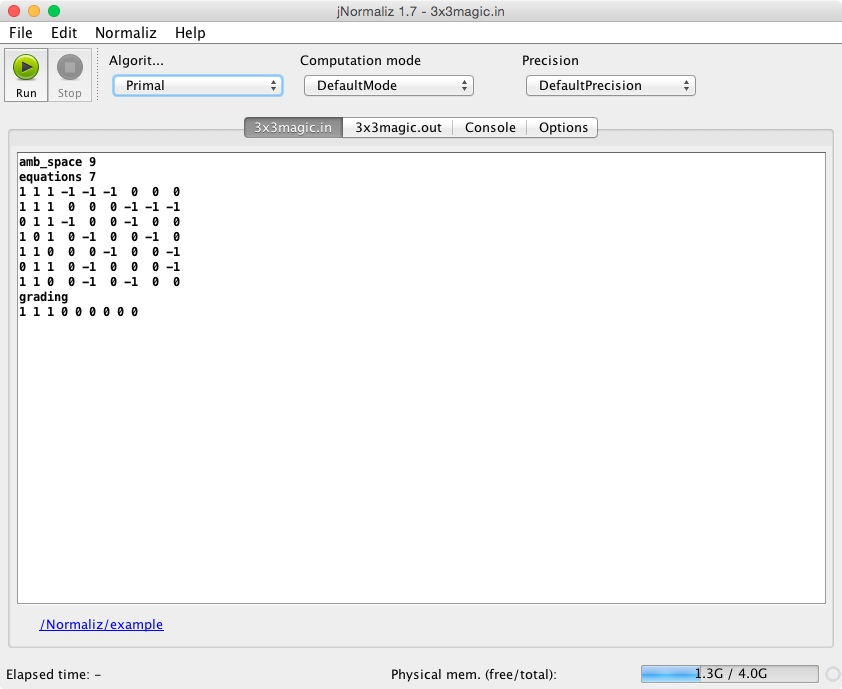
\includegraphics[width = 80 mm, bb=0 0 690 560]{jNormaliz.jpg}\\%width = 80 mm, bb=0 0 689 430
  \caption{\jNormaliz+}\label{new}
\end{figure}
In the \jNormaliz+ file dialogue choose one of the input files
in the subdirectory \ttt{example}, say \ttt{small.in}, and
press \ttt{Run}. In the console window you can watch \Normaliz+
at work. Finally inspect the output window for the results.

The menus and dialogues of \jNormaliz+ are self explanatory, but you
can also consult the documentation \cite{AI} via the help menu.

If the executables prepared cannot be run on your system, then
you can  compile \Normaliz+ yourself (see Section
\ref{Compile}).

Moreover, one can, and often will, run \Normaliz+ from the
command line. This is explained in Section \ref{options}.

If 64 bit integer precision is not sufficient, then one can
switch \jNormaliz+ to infinite precision (or use the option
\texttt{-B} from the command line). Then \Normaliz+ has no
restrictions on the integer precision. See Section
\ref{NumLim}. (The integer precision has nothing to do with the
address width (32 bit or 64 bit) of your operating system.)


%%%%%%%%%%%%%%%%%%%%%%%%%%%%%  INPUT  %%%%%%%%%%%%%%%%%%%%%%%%%%%%%
\section{The input file}\label{input}

The input file \ttt{<projectname>.in} consists of one or
several matrices. Each matrix is built as follows:

\begin{arab}
\item The first line contains the number of rows $m$.
\item The second contains the number of columns $n$.
\item The next $m$ lines of $n$ integers each contain the rows.
\item The last line contains a single number or word
    specifying the type of input the matrix presents.
\end{arab}

At the moment there are three major types of input matrices,
namely \emph{generators}, \emph{constraints}, and
\emph{relations}. An additional type is \emph{grading}.

For each input type we specify two lattices: the \emph{ambient
lattice} $\AA$ to which the input data refer and the
\emph{essential lattice} $\EE\subset \AA$ with respect to which
all data are computed.

In this section we assume that \Normaliz+ is run in a computation
mode in which the Hilbert basis is actually computed. (See Section
\ref{options} for computation modes.)

\subsection{Generators}

The generator types are 0, 1, 2 and 3. If a matrix of one of
these types is in the input file, then it must be the only
matrix in the file, unless a grading has been added.

\subsubsection{Type 0, \ttt{integral\_closure}}

The rows of an $m\times n$ matrix of type 0 represent $m$ vectors in
the ambient lattice $\AA=\ZZ^n$. The essential lattice $\EE$ is the
smallest direct summand of $\ZZ^n$ that contains the vectors in the
matrix.

The vectors are considered as a system of generators $\cG$ of a
cone $C$, and \Normaliz+ computes the Hilbert basis of $C$ with
respect to $\EE$ (or, equivalently,  $\ZZ^n$).

The nomenclature \ttt{integral\_closure} is explained by the
fact that the Hilbert basis generates the integral closure of
the monoid $\ZZ_+\cG$ in $\ZZ^n$.

A simple example:
\begin{myverb}
\begin{Verbatim}
Input            Hilbert basis
3                1 0
2                0 1
2 0
1 1
0 2
integral_closure
\end{Verbatim}
\end{myverb}
In this example, the three input vectors clearly generate the
positive orthant $\RR_+^2$ in $\RR^2$, and the two unit vectors
clearly are the Hilbert basis of $\RR_+^2\cap\ZZ^2$.

Example input files: \ttt{rproj2.in}, \ttt{small.in}.

\subsubsection{Type 1,
\ttt{normalization}}\label{normalization}

The matrix is interpreted as in type 0, however $\EE$ is chosen as
the sublattice of $\ZZ^n$ generated by $\cG$.

The choice of the name \ttt{normalization} indicates that
\Normaliz+ computes the normalization of the monoid $\ZZ_+\cG$.
(The computation of such normalizations was the original goal
of \Normaliz+, hence the name.)

We choose the same input vectors as above, but change the type to
\ttt{normalization}:
\begin{myverb}
\begin{Verbatim}
Input            Hilbert basis
3                2 0
2                1 1
2 0              0 2
1 1
0 2
normalization
\end{Verbatim}
\end{myverb}
The cone has not changed, but the lattice has: $\EE$ is now the
sublattice of $\ZZ^2$  of all $(z_1,z_2)$ with $z_1+z_2\equiv 0
\mod 2$.

Example input files: \ttt{rafa2416.in}, \ttt{A443.in},

\subsubsection{Type 2, \ttt{polytope}}

The rows of the matrix are interpreted as integral points of a
lattice polytope in $\RR^n$, which is their convex hull.

The cone $C$ is the cone over the polytope, i.e.\ the cone with apex
$0$ in $\RR^{n+1}$ generated by the vectors $(x,1)$ where $x$
represents a row of the input matrix. We want to compute the \emph{Ehrhart
monoid} $C\cap \ZZ^{n+1}$.

The lattice $\AA$ is $\ZZ^{n+1}$, and $\EE$ is the smallest
direct summand of $\AA$ containing the generators of $C$.

Type 2 is only a variant of type 0. One obtains the same results as
in type 0 with the extended vectors $(x,1)$ as input.

\emph{Note:} In previous versions, the text in the output file
was adapted to the polytopal situation. Since 2.8
\ttt{polytope} is only an input variant of type 0.

Example input files: \ttt{polytop.in}, \ttt{FortuneCookie.in},
\ttt{lo6.in}.

\subsubsection{Rational polytopes}\label{rat_pol_in}

\Normaliz+ has no special input type for rational polytopes.
In order to process them one uses type 0 together with a
grading. Suppose the polytope is given by vertices
$$
v_i=(r_{i1},\dots,r_{in}),\qquad i=1,\dots,m,\ r_{ij}\in\QQ.
$$
Then we write $v_i$ with a common denominator:
$$
v_i=\biggl(\frac{p_{i1}}{q_i},\dots,\frac{p_{in}}{q_i}\biggr),
\quad p_{ij},q_i\in\ZZ,\ q_i>0.
$$
The generator matrix is given by the rows
$$
\widetilde v_i=(p_{i1},\dots,p_{in},q_i),\quad i=1,\dots,m.
$$
We must add a grading since \Normaliz+ cannot recognize it
without help (unless all the $q_i$ are equal). The grading
vector has coordinates $(0,\dots,0,1)$. See \ref{grading} below
for general information on gradings.

Let us look at a concrete example (contained in \ttt{rational.in}),
the triangle $P$ with vertices
$$
(1/2,1/2),\ (-1/3,-1/3),\ (1/4,-1/2).
$$
In order to apply \Normaliz+ to it one uses the following
input:
\begin{myverb}
\begin{Verbatim}
3
3
1 1 2
-1 -1 3
1 -2 4
integral_closure
1
3
0 0 1
grading
\end{Verbatim}
\end{myverb}
The output will be discussed in \ref{rat_pol_out}.

\subsubsection{Type 3, \ttt{rees\_algebra}}

In this type the input vectors are considered as exponent
vectors of the generators of a monomial ideal $I$ in the
polynomial ring $K[X_1,\dots,X_n]$. \Normaliz+ computes the
normalization of the Rees algebra of the ideal $I$ (see
\cite{BH} for the notion of Rees algebra.) This is a monomial
subalgebra of the extended polynomial ring $K[X_1,\dots,X_n,T]$
with an auxiliary variable $T$. \Normaliz+ computes the
exponent vectors in $\ZZ^{n+1}$ of the system of generators.
For an example, see Section \ref{Examples}.

In type $3$ one has $\AA=\EE=\ZZ^{n+1}$.

Example input file: \ttt{rees.in}.

\subsubsection{Preparation of the generators}

After the coordinate transformation to the lattice $\EE$,
\Normaliz+ divides each generator by the greatest common
divisor of its components. For example, the extreme rays listed
will always be such $\EE$-primitive vectors (re-transformed to
$\AA$ where they may not be primitive).

If a grading is present, the generators will be sorted by
degree in ascending order. Those of the same degree will remain
sorted as in the input file (or the result of a previous
computation).

\subsection{Constraints}

Inequalities, equations, and congruences defining the cone and
the lattice are called \emph{constraints}. Matrices
representing them are of types 4, 5 and 6. All three types can
be present in the input file, and there can be several matrices
of each type. The order does not matter. Matrices of the same
type will be concatenated. The numbers of columns must of
course match: for the ambient lattice $\ZZ^n$ the matrices of
types 4 and 5 must have $n$ columns, and those of type 6 must
have $n+1$ columns.

If there is no matrix of type 4, then it is assumed that the
user wants to compute the nonnegative solutions of the system
represented by the matrices of type 5 and/or 6. The input file
is therefore compatible with the types 4 and 5 of previous
versions of \Normaliz+.

\subsubsection{Type 4, \ttt{hyperplanes}}

A row $(\xi_1,\dots,\xi_n)$ of the input matrix of type 4 represents
an inequality
$$
\xi_1x_1+\dots+\xi_nx_n\ge 0
$$
for the vectors $(x_1,\dots,x_n)$ of $\RR^n$.

Example:
\begin{myverb}
\begin{Verbatim}
Input            Hilbert basis
2                0 -1
2                1  1
1 0
1 -1
hyperplanes
\end{Verbatim}
\end{myverb}
\Normaliz+ has computed the Hilbert basis of the cone defined
by the inequalities $x_1\ge 0$ and $x_1-x_2\ge 0$ with respect
to the lattice $\ZZ^2$.

Example input file: \ttt{Condorcet.in}

\subsubsection{Sign inequalities}

There is a shortcut for the  input of inequalities $x_i\ge 0$
or $x_i\le 0$. The input matrix of type \ttt{signs} has format
$1\times n$ and the entries of its single row are in
$\{-1,0,1\}$:
\begin{itemize}
\item[$-1$] stands for $x_i\le 0$,
\item[$1$] stands for $x_i\ge 0$,
\item[$0$] indicates that the sign of $x_i$ is not
    restricted.
\end{itemize}

Example:
\begin{myverb}
\begin{Verbatim}
1
4
1 -1 0 1
signs
\end{Verbatim}
\end{myverb}
In this example we require that $x_1,x_4\ge 0$ and $x_2\le 0$.

Example input file: \ttt{Condorcet.in}

\subsubsection{Polytopes by inequalities}
\Normaliz+ has no special input type for polytopes defined by
inequalities since they can easily be specified via type 4.
Suppose the polytope is given by inequalities
$$
\alpha_{i_1}x_1+\dots+\alpha_{in}x_n\ge \beta_i,\quad i=1,\dots,m,\ \alpha_{ij},\beta_i\in \ZZ.
$$
Then we homogenize the inequalities in the form
$$
\alpha_{i_1}x_1+\dots+\alpha_{in}x_n-\beta_ix_{n+1}\ge0,
$$
and use type 4 for them in connection with the grading vector
$(0,\dots,0,1)$.

The file \ttt{poly\_ineq.in} contains
\begin{myverb}
\begin{Verbatim}
3
3
2  7 3
-8 2 3
1 -1 0
hyperplanes
1
3
0 0 1
grading
\end{Verbatim}
\end{myverb}
It reproduces the triangle that we have discussed in
\ref{rat_pol_in}.

\subsubsection{Type 5, \ttt{equations}}

A row $(\xi_1,\dots,\xi_n)$ of the input matrix of type 5 represents
an equation
$$
\xi_1x_1+\dots+\xi_nx_n=0
$$
for the vectors $(x_1,\dots,x_n)$ of $\RR^n$.

Example:
\begin{myverb}
\begin{Verbatim}
Input            Hilbert basis
1                2 0 1
3                0 2 1
1 1 -2           1 1 1
equations
\end{Verbatim}
\end{myverb}
If the input file contains no further matrices, \Normaliz+ has
computed the Hilbert basis of the subcone of $\RR_+^3$ defined
by the equation $x_1+x_1-2x_3= 0$.

Example input files: \ttt{4x4.in}, \ttt{5x5.in}.

\subsubsection{Type 6, \ttt{congruences}}

We consider the rows of a matrix of type 6 to have length $n+1$.
Each row $(\xi_1,\dots,\xi_n,c)$ represents a congruence
$$
\xi_1z_1+\dots+\xi_nz_n\equiv 0 \mod c
$$
for the elements $(z_1,\dots,z_n)\in\ZZ^n$.

Example:
\begin{myverb}
\begin{Verbatim}
Input            Hilbert basis
1                2 0
3                1 1
1 1 2            0 2
congruences
\end{Verbatim}
\end{myverb}
If no other matrix is in the input file, then \Normaliz+
computes the Hilbert basis of the positive orthant intersected
with the lattice of all integral vectors $(z_1,z_2)$ such that
$z_1+z_2\equiv 0 \mod 2$ and the result is the same as in
\ref{normalization} above.

Example input file: \ttt{3x3magiceven.in}.

\subsubsection{The constraints combined}

Let $L$ be the sublattice of $\ZZ^n$ that consists of the
solutions of the system of congruences defined by the input
matrix of type \ttt{congruences}. ($L=\ZZ^n$ if there is no
such matrix). Moreover let $A$ be the matrix of type
\ttt{hyperplanes}  (combined with the matrix representing the
\ttt{signs}) and $B$ be the matrix of type \ttt{equations}.
Then the cone $C$ is given by
$$
C=\{x\in\RR^n: Ax\ge 0,\ Bx= 0\}.
$$
and the Hilbert basis of $C\cap L$ is computed.

The ambient lattice $\AA$ is $\ZZ^n$, and the essential lattice
is $\EE=L\cap \RR C$.

If there is no matrix of type \ttt{equations}, then the system
of equations is empty, satisfied by all vectors of $\RR^n$.

Note that there is always a matrix of type \ttt{hyperplanes},
either explicitly in the input, or implicitly, namely the
$n\times n$ unit matrix, if there is no matrix of type
\ttt{hyperplanes} or \ttt{signs} in the input file (but one of
type \ttt{equations} or \ttt{congruences}).

See Section \ref{magiceven} for an example combining types
\ttt{equations} and \ttt{congruences}.

Example input file: \ttt{3x3magiceven.in}.


\subsection{Relations}\label{relations}

Relations are another type of constraints. They do not select a
sublattice of $\ZZ^n$ or a subcone of $\RR^n$, but define a
monoid as a quotient of $\ZZ_+^n$ modulo a system of
congruences (in the semigroup sense!).

Let $U$ be a subgroup of $\ZZ^n$. Then the natural image $M$ of
$\ZZ_+^n\subset\ZZ^n$ in the abelian group $G=\ZZ^n/U$ is a
submonoid of $G$. In general, $G$ is not torsionfree, and
therefore $M$ may not be an affine monoid. However the image
$N$ of $M$ in the lattice $L=G/\textup{torsion}$ is an affine
monoid. \Normaliz+ chooses an embedding
$L\hookrightarrow\ZZ^r$, $r=n-\rank U$, such that $N$ becomes a
submonoid of $\ZZ_+^r$. In general there is no canonical choice
for such an embedding, but one can always find one, provided
$N$ has no invertible element except $0$. The ambient lattice
is then $\AA=\ZZ^r$, and the essential lattice is $L$, realized
as a sublattice of $\AA$.

The typical starting point is an ideal $J\subset
K[X_1,\dots,X_n]$ generated by binomials
$$
X_1^{a_1}\cdots X_n^{a_n}-X_1^{b_1}\cdots X_n^{b_n}.
$$
The image of $K[X_1,\dots,X_n]$ in the residue class ring of
the Laurent polynomial ring $S=K[X_1^{\pm1},\dots,X_n^{\pm1}]$
modulo the ideal $JS$ is exactly the monoid algebra $K[M]$ of
the monoid $M$ above if we let $U$ be the subgroup of $\ZZ^n$
generated by the differences
$$
(a_1,\dots,a_n)-(b_1,\dots,b_n).
$$

Ideals of type $JS$ are called lattice ideals if they are
prime. Since \Normaliz+ automatically passes to
$G/\textup{torsion}$, it replaces $JS$ by the smallest lattice
ideal containing it.

\subsubsection{Type 10, \ttt{lattice\_ideal}}

The rows of the input matrix of type 10 are interpreted as
generators of the subgroup $U$, and \Normaliz+ performs the
computation as just explained.

As an example we consider the binomials $X_1X_3-X_2^2$,
$X_1X_4-X_2X_3$:
\begin{myverb}
\begin{Verbatim}
Input            Hilbert basis
2                3 0
4                2 1
1 -2  1 0        1 2
1 -1 -1 1        0 3
lattice_ideal
\end{Verbatim}
\end{myverb}
In this example $\ZZ^4/U$ is torsionfree, but we can replace each
of the vectors in the input matrix by a nonzero integral
multiple without changing the result.

Type 10 cannot be combined with any other input type (except
\ttt{grading})---such a combination would not make sense.

Example input file: \ttt{lattice\_ideal.in}.


\subsection{Gradings}\label{grading}

\Normaliz+ can compute the Hilbert series  and the Hilbert
(quasi)polynomial of a graded monoid. A \emph{grading} of a
monoid $M$ is simply a homomorphism $\deg:M\to\ZZ^g$ where
$\ZZ^g$ contains the degrees. The \emph{Hilbert series} of $M$
with respect to the grading is the formal Laurent series
$$
H(T)=\sum_{d\in \ZZ^g} \#\{x\in M: \deg x=d\}T_1^{d_1}\cdots T_g^{d_g},
$$
provided all sets $\{x\in M: \deg x=d\}$ are finite.

At the moment, \Normaliz+ can only handle the case $g=1$. A
$\ZZ$-valued grading can be specified in two ways:
\begin{arab}
\item \emph{explicitly} by including a grading in the input, or
\item \emph{implicitly}. In this case \Normaliz+ checks whether
    the extreme integral generators of the monoid lie in an
    (affine) hyperplane $A$. If so, then the (unique) primitive
    $\ZZ$-linear form $\lambda$ that affords an equation
    $\lambda(x)=b$ for $A$ is used as the grading.
\end{arab}

The basic fact about $H(t)$ in the $\ZZ$-graded case is that it
is the Laurent expansion of a rational function at the origin:
\begin{equation}
H(t)=\frac{R(t)}{(1-t^e)^r},\qquad R(t)\in\ZZ[t],\label{raw}
\end{equation}
where $r$ is the rank of $M$ and $e$ is the least common multiple
of the degrees of the extreme integral generators of the cone.

Usually one can find denominators for $H(t)$ of much lower
degree than in equation \eqref{raw}, and \Normaliz+ tries to
give a more economical presentations of $H(t)$ as a quotient of
two polynomials. One should note that it is not clear what the
most natural presentation of $H(t)$ is in general (when $e>1$).
We discuss this problem in \cite[Section 4]{BIS} and in
\ref{rat_pol_out}. The examples in Section \ref{Examples},
especially \ref{rat_pol_out} and \ref{magiceven}, may serve as
an illustration.

A rational cone $C$ and a grading together define the rational
polytope $P=C\cap A_1$ where $A_1=\{x:\deg x=1\}$. In this
sense the Hilbert series is nothing but the Ehrhart series of
$P$.

\emph{Note:} In previous versions we used \emph{height} as a
synonym for \emph{degree}.

A grading is explicitly specified by an $1\times n$ matrix for
cones embedded in $\RR^n$, and its type is fixed by the
attribute \ttt{grading}, for example
\begin{myverb}
\begin{Verbatim}
1
2
3 2
grading
\end{Verbatim}
\end{myverb}
We have not assigned a numerical type to matrices (effectively,
vectors) specifying the grading.

\Normaliz+ checks whether all generators of the monoid have
positive degree.

Before \Normaliz+ can apply the degree, it must be restricted
to the effective lattice $\EE$. Even if the entries of the
grading vector are coprime, it often happens that all degrees
of vectors in $\EE$ are divisible by a greatest common divisor
$ d>1$. Then $d$ is extracted from the degrees, and it will
appear as \ttt{denominator} in the output file.

Special rules apply to some input types that we explain in the
following.

\subsubsection{\ttt{polytope}}
Cones defined by lattice polytopes always have an implicit
grading in which the lattice points in the polytope have degree
$1$ (roughly speaking). Therefore it is not possible to use an
explicit grading together with this input type.

If it should be necessary to apply a different grading, then
one converts the input of type \ttt{polytope} to
\ttt{integral\_closure} by appending \ttt{1} to each row of the
input matrix and adds the grading to be used.

\subsubsection{\ttt{rees\_algebra}} Suppose that the rows of the
input matrix specify vectors of length $n$. Then these are
embedded into $\RR^{n+1}$, and therefore the grading must have
$n+1$ components. Example:
\begin{myverb}
\begin{verbatim}
3
3
0 1 2
2 0 2
1 1 1
rees_algebra
1
4
1 1 1 -1
grading
\end{verbatim}
\end{myverb}

Note that the Rees algebra has an implicit grading if and only
if all the monomials have the same total degree, say $g$. Then
the grading vector chosen automatically is
$(1,\dots,1,-(g-1))$.

\subsubsection{\ttt{lattice\_ideal}}

In this case the unit vectors correspond to generators of the
monoid. Therefore the degrees assigned to them must be
positive. Moreover, the vectors in the input represent binomial
relations, and these must be homogeneous. In other words, both
monomials in a binomial must have the same degree. This amounts
to the condition that the input vectors have degree $0$.
\Normaliz+ checks this condition. Example:

\begin{myverb}
\begin{verbatim}
1
4
1 1 -1 -1
lattice_ideal
1
4
1 2 1 2
grading
\end{verbatim}
\end{myverb}

\subsection{Pointedness}

For Hilbert basis computations and triangulations \Normaliz+
requires the cone to be pointed ($x,-x\in C\implies x=0$).
Whenever the condition of pointedness is violated at a step
where it is crucial, \Normaliz+ will stop computations.

Pointedness is checked by testing whether the dual cone of $C$
is full dimensional, and if not, then the constructor of the
cone complains as follows:

\begin{Verbatim}
Full Cone error: Matrix with rank = number of columns needed in
the constructor of the object Full_Cone. Probable reason: Cone
not full dimensional(<=> dual cone not pointed)!
\end{Verbatim}

\subsection{The zero cone}\label{zero}

The zero cone with an empty Hilbert basis is a legitimate
object for \Normaliz+. Nevertheless a warning message is issued
if the zero cone is encountered.

\subsection{Additional input file for NmzIntegrate}

\NmzIntegrate+, whether called by \Normaliz+ or from the command
line, needs an input file \ttt{<projectname>.pnm} that contains
the polynomial for which the generalized Ehrhart series or the
integral is to be computed. See \cite{NmzInt}.


%%%%%%%%%%%%%%%%%%%%%%%%%%%%%  RUNNING  %%%%%%%%%%%%%%%%%%%%%%%%%%%%%
\section{Running Normaliz}\label{options}

The simplest way to call \Normaliz+ from the command line is
\begin{center}
\ttt{normaliz <projectname>}
\end{center}
for example
\begin{center}
\ttt{normaliz rafa2416}
\end{center}
The project name is \ttt{rafa2416}. \Normaliz+ reads the input
file \ttt{rafa2416.in} (hopefully existing), computes
everything it can compute, and writes the output to
\ttt{rafa2416.out}.

The full syntax for calling \Normaliz+ from the command line is
\begin{center}
\ttt{normaliz [-stvnhpN1dcBefaT] [-x=<T>] [<projectname>]}
\end{center}
where the options and \ttt{<projectname>} are optional. (We assume
that the executable \ttt{normaliz} or \ttt{normaliz.exe} is in the
search path. Otherwise you have to prefix it with a suitable
relative or absolute path.) If no \ttt{<projectname>} is given, the
program will ask you for it or display a help screen.

The option \ttt{-x} differs from the other ones: \ttt{<T>}
represents a positive number assigned to \ttt{-x}; see
Section \ref{exec}.

The help screen can also be displayed by \ttt{normaliz -?}.

\Normaliz+ will look for \ttt{<projectname>.in} as input
file.

For example, if you input the command
\begin{center}
\ttt{normaliz -c -p -a -T rafa2416} \qquad or\qquad
\ttt{normaliz -cpaT rafa2416}
\end{center}
then the program will take the file \ttt{rafa2416.in} as input,
control data will be displayed on your terminal, the support
hyperplanes, the triangulation, the multiplicity, the Hilbert
series and the Hilbert (quasi)polynomial will be computed and
all the possible output files will be produced.

If you inadvertently typed \ttt{rafa2416.in} as the project
name, then \Normaliz+ will first look for \ttt{rafa2416.in.in}
as the input file. If this file doesn't exist,
\ttt{rafa2416.in} will be loaded.

In the following we explain the various options of Normaliz.
The full text names given appear in the help screen as well as
in the menus of \jNormaliz+ which allows you to choose options
interactively.

{\bf The default computation mode is \ttt{-h}. All options that
can be activated are switched off by default.}

Adding a pure output option, namely \ttt{-f} or \ttt{-a}, or an
option controlling execution does not change the computation
mode.

\emph{Note:} (1) In 2.7 and earlier versions the default
computation mode was \ttt{-n}. The change to \ttt{-h} reflects
that the extra time for the computation of the Hilbert series
can be neglected now (actually, already in 2.7). The choice of
\ttt{-h} ensures that \Normaliz+ computes all the information
accessible to it.

(2) In version 2.8 and earlier, options were evaluated from
left to right. Therefore the last of mutually exclusive options
was used. Now options can be accumulated.


\subsection{Computation modes}

\subsubsection{Support hyperplanes and extreme rays}

The least that \Normaliz+ can do is
\begin{itemize}
\itemtt[-s] \ttt{support hyperplanes}: only the support
    hyperplanes of the cone under consideration and the
    extreme rays are computed.
\end{itemize}

\subsubsection{Modes with partial triangulation}

For the computation of Hilbert bases and/or degree $1$ elements
it is enough to use a partial triangulation (see \cite{BHIKS}).
The following two computation modes take advantage of this
fact:

\begin{itemize}
\itemtt[-N] \ttt{Hilbert basis}: includes \ttt{-s} and
    computes the Hilbert basis.
\item [-1] \ttt{degree 1 elements}: includes \ttt{-s}, only
    degree 1 elements are computed. (This is the fastest
    mode for computing the lattice points in a polytope.)
\end{itemize}


\subsubsection{Modes with full triangulation}

The following modes form an ascending chain. All of them
compute a full triangulation:

\begin{itemize}
\itemtt[-t] \ttt{triangulation}: in addition to the support
    hyperplanes the triangulation is computed, but not
    evaluated (it can be written to the output). Why
    \texttt{-t} is nevertheless useful will be explained in
    Section \ref{Large}.
\itemtt[-v] \ttt{volume}: includes \ttt{-t}. Now \Normaliz+
    evaluates the triangulation and computes the
    multiplicity (or normalized volume) if a grading is
    available.
\itemtt[-n] \ttt{Hilbert basis volume}: includes \ttt{-v}
    and \Normaliz+ computes the Hilbert basis.
\itemtt[-h] \ttt{Hilbert basis series}:  includes \ttt{-n}.
    If a grading is given, \Normaliz+ computes the Hilbert
    series and the Hilbert (quasi)poly\-nomi\-al. This
    computation mode yields the maximum information
    \Normaliz+ can produce.
\end{itemize}

If only the Hilbert series is to be computed, then one uses
\begin{itemize}
\itemtt[-q] \ttt{Hilbert series} or
\item[-p] \ttt{Hilbert series degree 1 elements}.This mode
    includes \ttt{-1}.
\end{itemize}

Both \ttt{-p} and \ttt{-q} include \ttt{-v}.

Note: once the Hilbert series is computed, the computation of
the degree $1$ elements does not cost much extra time. It may
however cause a substantial amount of output.

\subsubsection{The dual algorithm}

If a cone is defined by constraints, it is often (but not
always) faster to use a Hilbert basis algorithm originally due
to Pottier \cite{Po} that we call the \emph{dual} algorithm, in
contrast to the \emph{primal} (triangulation based) algorithm
of \Normaliz+. (See \cite{BI} for our version of the dual
algorithm.) The dual algorithm is invoked by

\begin{itemize}
\itemtt[-d] \ttt{dual}
\end{itemize}

By itself, the dual algorithm computes only Hilbert bases (and
degree $1$ elements if a grading is given), but it can be
combined with the other options. For example, \ttt{-dq} starts
a Hilbert basis computation with the dual algorithm, followed
by a computation of the Hilbert series.

The dual algorithm can be used with all input types. See
Section \ref{PerPar} for a comparison of performance on various
examples.

\subsubsection{What option do I use \dots}

The following table gives an overview of the computation
options introduced so far (except \ttt{-t}).
\begin{center}
\begin{tabular}{l|c|c|c|}
&No enumera-&&Hilbert\\
&tive data&multiplicity&series\\
\hline
No vectors&&&\\
or points&\ttt{-s}&\ttt{-v}&\ttt{-q}\\
\hline
degree 1&&&\\
elements &\ttt{-1}&\ttt{-v1}&\ttt{-p}\\
\hline
Hilbert &\ttt{-d}&&default,\\
basis &\ttt{-N}&\ttt{-n}&\ttt{-h}\\
\hline
\end{tabular}
\end{center}

As mentioned above, combinations with \ttt{-d} are possible and
may be useful.

Note: at present, it is not possible to restrict the dual
algorithm to the computation of degree $1$ elements.


\subsubsection{Modes calling NmzIntegrate}

\NmzIntegrate+ is an independent executable, but it can be
called by \Normaliz+. The options are exactly those that would
be used for a command line call of \NmzIntegrate+:

\begin{itemize}
\itemtt[-E] \ttt{Generalized Ehrhart series}: computation
    of generalized Ehrhart series,
\itemtt[-L] \ttt{Leading coefficient}: computation of
    leading coefficient of generalized Ehrhart
    quasipolynomial,
    \itemtt[-I] \ttt{Integral}: computation of Lebesgue
        integral.
\end{itemize}

See \cite{NmzInt} for the details of \NmzIntegrate+. The
options \ttt{-c} and \ttt{-x=<T>} are forwarded to
\NmzIntegrate+.

The option \ttt{-E} contains \ttt{-y}, and \ttt{-I} and
\ttt{-L} both contain \ttt{-T}. See Section \ref{outcontrol}
for \ttt{-T} and \ttt{-y}.


\subsection{Control of output files}\label{outcontrol}

In the default setting \Normaliz+ writes only the output file
\ttt{<projectname>.out}. The amount of output files can be
increased as follows:
\begin{itemize}
\itemtt[-f] \Normaliz+ writes the additional output files
    with suffixes \ttt{gen}, \ttt{cst}, and \ttt{inv},
    provided the data of these files have been computed.
\itemtt[-a] includes \ttt{-f}, \Normaliz+ writes all
    available output files except the triangulation or the
    Stanley decomposition.
\itemtt[-T] \Normaliz+ writes the triangulation and the
    file with suffix \ttt{inv}.
\itemtt[-y] \Normaliz+ writes the Stanley decomposition and
    the file with suffix \ttt{inv}.
\end{itemize}

Note that \ttt{-T} and \ttt{-y} do not only write the data of
the triangulation or Stanley decomposition to the output, but
also force their computation, even if there is no other reason
to compute them.

In order to see all available output files one uses \ttt{-aTy}.

The triangulation and the Stanley decomposition are treated
separately since they can become very large and may exhaust
memory if they must be stored for output.

For the list of potential output files and their interpretation
see Section \ref{optionaloutput}.


\subsection{Control of execution}\label{exec}

The options that control the execution are:

\begin{itemize}
\itemtt[-c] activates the verbose (``control'') behavior of
    \Normaliz+ in which \Normaliz+ writes additional
    information about its current activities to the
    standard output.
\itemtt[-e] activates the overflow error check of
    \Normaliz+. Ignored if used with -B.
\itemtt[-B] Switches \Normaliz+ to infinite precision.
\itemtt[-x=<T>] Here \ttt{<T>} stands for a positive
    integer limiting the number of threads that \Normaliz+
    is allowed access on your system. The default value is
    set by the operating system. If you want to run
    \Normaliz+ in a strictly serial mode, choose
    \ttt{-x=1}.
\end{itemize}

The number of threads can also be controlled by the environment
variable \verb+OMP_NUM_THREADS+. See Section \ref{PerPar} for
further discussion.

\subsection{Numerical limitations}\label{NumLim}

Even in low dimensions, the range of 64 bit integers may not be
sufficient for the computations of \Normaliz+. Therefore
\texttt{normaliz} can be switched to infinite precision by the
option \texttt{-B}.

Computations with \ttt{-B} typically run about 5 times slower than
those without it. In examples that look critical, it may be useful
first to try \ttt{normaliz} without \texttt{-B}, but with the error
check option activated. This costs time, too, but hardly more than
50\% extra.

The user should run the example \ttt{critical64.in} in the
subdirectory \ttt{examples} with \ttt{normaliz -e} in order to
see the failure of 64 bit arithmetic. (Running it with \ttt{-B}
takes a while and requires much memory.)

\subsection{Obsolete options}

The options \ttt{-i} and \ttt{-m} of version 2.2 have become
obsolete. They will be ignored if present.

The options \texttt{-SVHP} of versions 2.5 and 2.7 are now
synonymous with\texttt{-svhp} and can still be used.




%%%%%%%%%%%%%%%%%%%%%%%%%%%%%  OUTPUT  %%%%%%%%%%%%%%%%%%%%%%%%%%%%%
\section{The output file}\label{output}

The data you will find in the output file depend on the input
type and on the computation mode. The output file starts with
an ``abstract'' that collects various numerical and qualitative
data, for example the number of elements in the Hilbert basis.
The lists of vectors, equations etc.\ follow the abstract.

The output file \ttt{<projectname>.out} will contain the
following data as far as computed:

\begin{itemize}
\item only for type 10: the original system of generators
    (see below);
\item  the Hilbert basis $H$ computed;
\item the extreme rays of the cone $C$ generated by $H$;
\item the rank of the lattice $\EE$;
\item the index of the lattice generated by the original input vectors in $\EE$;
\item the support hyperplanes of $C$;
\item a system of equations defining the vector space generated by
$C$;
\item a system of congruences defining $\EE$ as a sublattice of
$\AA$ (together with the equations);
\item the number of simplicial cones in the triangulation
    and the sum of the absolute values of their
    determinants.
\end{itemize}
In the presence of a grading the following extra data may be
printed:
\begin{itemize}
\item the linear form defining the degree;
\item the degree $1$ elements of the Hilbert basis;
\item the multiplicity;
\item the Hilbert series and the coefficients of the
    Hilbert (quasi)polynomial.
\end{itemize}

The degrees of the extreme rays are listed in the abstract. If
the whole Hilbert basis is of degree 1, this fact is indicated.
Moreover, \Normaliz+ tells you whether the original system of
generators contains the Hilbert basis by indicating whether the
original monoid is integrally closed.

Please note:

\begin{arab}
\item The equations and support hyperplanes \emph{together}
    define the cone $C$. While support hyperplanes will
    always be present (except for the zero cone), equations will
    only be printed if necessary, namely when $\dim
    C<\rank\AA$.

Similarly, congruences will only be printed if the lattice $\EE$
is not given by $\RR C\cap \AA$. This can only happen with
input matrices of type $1$ or $6$.

Even if the cone and the lattice are defined by constraints,
the inequalities, equations and congruences of the input will
in general not be reproduced, but replaced by an equivalent
system.

\item The extreme rays are given by the first points in $\EE$ on
them (the extreme integral generators with respect to $\EE$).

\item In order to lift the grading from
    $\EE$ to $\AA$ it may be necessary to replace it by a
    multiple (in order to avoid fractions as coefficients).
    The necessary factor appears as ``denominator''. The Hilbert series
    and the Hilbert (quasi)polynomial do always refer to the degree in $\EE$.

\item Input matrices of types 0, 1, 2 or 3 contain an explicit
    system of generators. For the other types $\neq 10$  the extreme rays
    computed by \Normaliz+ take their place. For type 10
    \Normaliz+ first computes the monoid $M$ generated by the
    residue classes of the canonical basis of $\ZZ^n$ (compare
    Section \ref{relations}), and they are considered the
    original system of generators.
\end{arab}


In type $=3$ (\ttt{rees\_algebra}), the data in the output file
refer to the integral closure $\Bar{\cR}$ of the Rees algebra.
In addition to what has been mentioned already, the following
data are computed:

\begin{itemize}
\item the generators of the integral closure of the ideal;
\item if the ideal is primary to the irrelevant maximal
    ideal, the multiplicity of the ideal (not to be
    confused with the multiplicity of the monoid).
\end{itemize}

%%%%%%%%%%%%%%%%%%%%%%%%%%%%%  EXAMPLES  %%%%%%%%%%%%%%%%%%%%%%%%%%%%%
\section{Examples}\label{Examples}

\subsection{Generators}

\subsubsection{Type 0, \ttt{integral\_closure}}

The file \ttt{rproj2.in} contains the following (here
typeset in 2 columns):

\begin{myverb}
\begin{Verbatim}
 16
  7
 1 0 0 0 0 0 0             1 0 1 0 1 0 1
 0 1 0 0 0 0 0             1 0 0 1 0 1 1
 0 0 1 0 0 0 0             1 0 0 0 1 1 1
 0 0 0 1 0 0 0             0 1 1 0 0 1 1
 0 0 0 0 1 0 0             0 1 0 1 1 0 1
 0 0 0 0 0 1 0             0 1 0 0 1 1 1
 1 1 1 0 0 0 1             0 0 1 1 1 0 1
 1 1 0 1 0 0 1             0 0 1 1 0 1 1
                           0
\end{Verbatim}
\end{myverb}

This means that we wish to compute the the cone $C$ generated
by the $16$ vectors
$$
(1,0,0,0,0,0,0)\,,\quad (0,1,0,0,0,0,0)\,,\quad \dots\,,\quad
(0,0,1,1,0,1,1)
$$
in $\RR^7$ with respect to the full lattice $\ZZ^7$, as indicated by
the final digit that specifies the type. (Actually, the vectors
generate the full lattice so that a replacement of type 0 by type 1
would not change anything.)

Running \ttt{normaliz} with no option (or option \ttt{-h},
\ttt{Hilbert basis series}) produces the file \ttt{rproj2.out}
which has the following content (partially typeset in 2 or 3
columns):

\begin{myverb}
\begin{Verbatim}
17 Hilbert basis elements                     multiplicity = 72
16 Hilbert basis elements of degree 1
16 extreme rays                               Hilbert series:
24 support hyperplanes                        1 9 31 25 6
                                              denominator with 7 factors:
rank = 7 (maximal)                            1: 7
index = 1
original monoid is not integrally closed      Hilbert polynomial:
                                              60 194 284 245 130 41 6
size of triangulation = 67                    with common denominator = 60
resulting sum of |det|s = 72

grading:
1 1 1 1 1 1 -2

degrees of extreme rays:
1: 16

Hilbert basis elements are not of degree 1

***********************************************************************

17 Hilbert basis elements:                 24 support hyperplanes:
 0 0 0 0 0 1 0                               0  0  0  1  0  0  0
 0 0 0 0 1 0 0                               0  0  0  0  1  0  0
 0 0 0 1 0 0 0                               0  0  0  0  0  1  0
 0 0 1 0 0 0 0                               0  0  0  0  0  0  1
 0 0 1 1 0 1 1                               0  0  1  0  0  0  0
 0 0 1 1 1 0 1                               0  1  0  0  0  0  0
 0 1 0 0 0 0 0                               0  1  1  0  0  1 -1
 0 1 0 0 1 1 1                               0  1  0  0  1  1 -1
 0 1 0 1 1 0 1                               0  1  0  1  1  0 -1
 0 1 1 0 0 1 1                               0  0  1  1  0  1 -1
 1 0 0 0 0 0 0                               0  1  1  1  1  1 -2
 1 0 0 0 1 1 1                               0  0  1  1  1  0 -1
 1 0 0 1 0 1 1                               1  0  0  0  0  0  0
 1 0 1 0 1 0 1                               1  1  1  1  1  1 -3
 1 1 0 1 0 0 1                               1  0  0  0  1  1 -1
 1 1 1 0 0 0 1                               1  0  0  1  0  1 -1
 1 1 1 1 1 1 2                               1  0  1  0  1  0 -1
                                             1  0  1  1  1  1 -2
16 extreme rays:                             1  1  1  0  0  0 -1
 1 0 0 0 0 0 0                               1  1  1  1  0  1 -2
 0 1 0 0 0 0 0                               1  1  0  1  0  0 -1
 0 0 1 0 0 0 0                               1  1  1  0  1  1 -2
 0 0 0 1 0 0 0                               1  1  1  1  1  0 -2
 0 0 0 0 1 0 0                               1  1  0  1  1  1 -2
 0 0 0 0 0 1 0
 1 1 1 0 0 0 1               16 degree 1 Hilbert basis elements:
 1 1 0 1 0 0 1                0 0 0 0 0 1 0
 1 0 1 0 1 0 1                0 0 0 0 1 0 0
 1 0 0 1 0 1 1                0 0 0 1 0 0 0       0 1 1 0 0 1 1
 1 0 0 0 1 1 1                0 0 1 0 0 0 0       1 0 0 0 0 0 0
 0 1 1 0 0 1 1                0 0 1 1 0 1 1       1 0 0 0 1 1 1
 0 1 0 1 1 0 1                0 0 1 1 1 0 1       1 0 0 1 0 1 1
 0 1 0 0 1 1 1                0 1 0 0 0 0 0       1 0 1 0 1 0 1
 0 0 1 1 1 0 1                0 1 0 0 1 1 1       1 1 0 1 0 0 1
 0 0 1 1 0 1 1                0 1 0 1 1 0 1       1 1 1 0 0 0 1
\end{Verbatim}
\end{myverb}

From this, we see that there are $17$ elements in the Hilbert
basis, of which 16 are of degree $1$, and $16$ extreme rays,
that the sublattice generated by the input vectors has index
$1$ in $\ZZ^7$, and that the corresponding support hyperplanes
are given by the linear forms $(0,0,0,1,0,0,0)$,
$(0,0,0,0,1,0,0)$, \dots, $(1,1,0,1,1,1,-2)$.

We are also given the information that there is a grading
(defined implicitly) and what it is. The multiplicity  with
respect to this grading is $72$. By definition, the
multiplicity is the $\EE$-normalized volume of the polytope
obtained by intersecting the cone with the hyperplane at degree
$1$.

The degrees of the extreme rays are given in multiset notation:
\begin{quote}
\ttt{1: 16}
\end{quote}
indicates that $16$ extreme rays have degree $1$.
(The input file contains no explicit grading. The implicitly
defined grading requires that all extreme rays have the same
degree, but it need not be $1$ as in this case.)

Since there is a grading, the degree 1 elements of the Hilbert
basis, the Hilbert series and Hilbert polynomial of the monoid
generated by the Hilbert basis are also computed. The Hilbert
series is given as a rational function. Its numerator
polynomial is
$$
1+9t+31t^2+25t^3+6t^4
$$
as we can see from the vector below the heading \ttt{Hilbert
series}. The denominator is given in multiset notation: \ttt{1:
7} specifies the denominator
$$
(1-t^1)^7.
$$
More general cases will be discussed in \ref{rat_pol_out} and
\ref{magiceven} below.

The Hilbert polynomial is given by
$$
P(k)=\frac{60}{60}+\frac{194}{60}k+\frac{284}{60}k^2+\frac{245}{60}k^3
+\frac{130}{60}k^4+\frac{41}{60}k^5+\frac{6}{60}k^6\,.
$$
The Hilbert polynomial gives the number of elements of degree
$k$, starting from degree $0$, as is always the case for normal
monoids. Note that the multiplicity $m$ can also be read from
the leading coefficient $c$ of the Hilbert polynomial:
\begin{equation}
c=\frac m{(r-1)!},\qquad r=\textup{rank},\label{multlead}
\end{equation}
in our case
$$
c=\frac1{10}=\frac{72}{720}.
$$

The lines
\begin{myverb}
\begin{Verbatim}
size of triangulation = 67
resulting sum of |det|s = 72
\end{Verbatim}
\end{myverb}
give some information about \Normaliz+' (not so hard) work: It
produced a triangulation of $67$ simplicial cones, and the sum
of the absolute values of the determinants of their generator
matrices is $72$. It is not surprising that this number equals
the multiplicity. This is always the case if only degree $1$
vectors appear in the generator matrix.

We omit an example of type 1 since it does not add anything new.

\subsubsection{Type 2, \ttt{polytope}}\label{latt_pol}

The file \ttt{polytop.in}:
\begin{myverb}
\begin{Verbatim}
 4
 3
 0 0 0
 2 0 0
 0 3 0
 0 0 5
 polytope
\end{Verbatim}
\end{myverb}

The Ehrhart monoid of the integral polytope with the $4$
vertices
$$
(0,0,0)\,,\quad (2,0,0)\,,\quad (0,3,0)\quad\text{ and }\quad (0,0,5)
$$
in $\RR^3$ is to be computed. (Note the last line, indicating the
polytope type 2.)

Running \ttt{normaliz} without an option (or option \ttt{-h}) produces the file \ttt{polytop.out}:

\begin{myverb}
\begin{Verbatim}
19 Hilbert basis elements                          multiplicity = 30
18 Hilbert basis elements of degree 1
4 extreme rays                                     Hilbert series:
4 support hyperplanes                              1 14 15
                                                   denominator with 4 factors:
rank = 4 (maximal)                                 1: 4
index = 30
original monoid is not integrally closed           Hilbert polynomial:
                                                   1 4 8 5
size of triangulation = 1                          with common denominator = 1
resulting sum of |det|s = 30

grading:
0 0 0 1

degrees of extreme rays:
1: 4

Hilbert basis elements are not of degree 1

***********************************************************************

19 Hilbert basis elements:     18 Hilbert basis elements of degree 1:
 0 0 5 1                        0 0 5 1
 0 3 0 1                        0 3 0 1
 2 0 0 1                        2 0 0 1
 0 0 0 1                        0 0 0 1
 0 1 3 1                        0 1 3 1
 0 1 2 1                        0 1 2 1
 0 1 1 1                        0 1 1 1
 0 1 0 1                        0 1 0 1
 0 0 4 1                        0 0 4 1
 0 0 3 1                        0 0 3 1
 0 0 2 1                        0 0 2 1
 0 0 1 1                        0 0 1 1
 0 2 0 1                        0 2 0 1
 0 2 1 1                        0 2 1 1
 1 0 0 1                        1 0 0 1
 1 0 1 1                        1 0 1 1
 1 0 2 1                        1 0 2 1
 1 1 0 1                        1 1 0 1
 1 2 4 2

4 extreme rays:                4 support hyperplanes:
 0 0 0 1                        -15 -10  -6  30
 2 0 0 1                          1   0   0   0
 0 3 0 1                          0   1   0   0
 0 0 5 1                          0   0   1   0
\end{Verbatim}
\end{myverb}

For the polytopal interpretation one must observe that all data
are in homogenized coordinates for which \Normaliz+ has
appended $1$  to the input vectors that (in this case) are the
vertices of the polytope. In the cone produced the lattice
points of the polytope are of degree $1$. Therefore the $18$
Hilbert basis elements of degree $1$ represent the lattice
points of the polytope, starting from $(0,0,5)$ and ending with
$(1,1,0)$. The extreme rays represent the $4$ vertices.

From the fact that there are $19$ Hilbert basis elements, but
only $18$ of degree $1$, we see that the lattice points in the
polytope do not yield the Hilbert basis of the Ehrhart monoid
(or the cone over the polytope).

That there is only one simplicial cone in the triangulation is
not surprising since our polytope is a simplex.

The support hyperplanes give us a description of the polytope
by inequalities: it is the solution of the system of the $4$
inequalities
$$ x_3\ge0\,,\quad
x_2\ge0\,,\quad x_1\ge0\quad\text{ and }\quad
15x_1+10x_2+6x_3\le30\,,
$$

The dimension of the polytope is $3$ since the cone over it has
dimension $4$. The polytope has $\ZZ^3$-normalized volume $30$
as indicated by the multiplicity.

The Ehrhart series (we use the more general term Hilbert
series) is
$$
\frac{1+14t+15t^2}{(1-t)^4}
$$
and its Ehrhart polynomial (again we use a more general term in
the output file) of the polytope is
$$
p(k)=1+4k+8k^2+5k^3\,.
$$

\subsubsection{A rational polytope}\label{rat_pol_out}

We want to investigate the Ehrhart series of the triangle $P$
with vertices
$$
(1/2,1/2),\ (-1/3,-1/3),\ (1/4,-1/2).
$$
The input file is \ttt{rational.in}. Running \Normaliz+ yields
the following output:

\begin{myverb}
\begin{verbatim}
8 Hilbert basis elements                   Hilbert series with cyclotomic denominator:
1 Hilbert basis elements of degree 1       -1 -1 -1 -3 -4 -3 -2
3 extreme rays                             cyclotomic denominator:
3 support hyperplanes                      1: 3  2: 2  3: 1  4: 1

rank = 3 (maximal)                         Hilbert quasi-polynomial of period 12:
index = 15                                   0:   48  28  15
original monoid is not integrally closed     1:   11  22  15
                                             2:  -20  28  15
size of triangulation   = 1                  3:   39  22  15
resulting sum of |det|s = 15                 4:   32  28  15
                                             5:   -5  22  15
grading:                                     6:   12  28  15
0 0 1                                        7:   23  22  15
                                             8:   16  28  15
degrees of extreme rays:                     9:   27  22  15
2: 1  3: 1  4: 1                            10:   -4  28  15
                                            11:    7  22  15
multiplicity = 5/8                         with common denominator = 48

Hilbert series:
1 0 0 3 2 -1 2 2 1 1 1 1 2
denominator with 3 factors:
1: 1  2: 1  12: 1


***********************************************************************

8 Hilbert basis elements:         3 extreme rays:
  1 -2  4                           1  1  2
 -1 -1  3                          -1 -1  3
  1  1  2                           1 -2  4
  0  0  1
  0 -1  3                         3 support hyperplanes:
  1  0  3                           2  7  3
  1 -1  4                          -8  2  3
  0 -2  5                           1 -1  0

                                  1 Hilbert basis elements of degree 1:
                                   0 0 1
\end{verbatim}
\end{myverb}
The $3$ extreme rays have reproduced the vertices (don't forget
that the last coordinate can be interpreted as a denominator),
and the $3$ support hyperplanes represent the $3$ inequalities
that define the polytope as an intersection of affine
halfspaces like in \ref{latt_pol}. The Hilbert basis element of
degree $1$ shows that there is a single lattice point in the
polytope, namely the origin $(0,0)$. Except that $P$ has
non-integral vertices now, these data are completely analogous
to those of the lattice polytope in \ref{latt_pol}.

The multiplicity is a rational number. Since in dimension $2$
the normalized area (of full-dimensional polytopes) is twice
the Euclidean area, we see that $P$ has Euclidean area $5/16$.

The Hilbert (or Ehrhart) function counts the lattice points in
$kP$, $k\in\ZZ_+$. The corresponding generating function is a
rational function $H(t)$ with numerator
$$
1+3t^3+2t^4-t^5+2t^6+2t^7+t^8+t^9+t^{10}+t^{11}+2t^{12}
$$
and denominator
$$
(1-t)(1-t^2)(1-t^{12}).
$$
As a rational function, $H(t)$ has degree $-3$. This implies
that $3P$ is the smallest integral multiple of $P$ that
contains a lattice point in its interior.

\Normaliz+ gives also a representation as a quotient of coprime
polynomials with the denominator factored into cyclotomic
polynomials. The multiset notation lists the orders of the
cyclotomic polynomials and their multiplicities. In this case
we have
$$
H(t)=-\frac{1+t+t^2+t^3+4t^4+3t^5+2t^6}{\zeta_1^3\zeta_2^2\zeta_3\zeta_4}
$$
where $\zeta_i$ is the $i$-th cyclotomic polynomial
($\zeta_1=t-1$, $\zeta_2=t+1$, $\zeta_3=t^2+t+1$,
$\zeta_4=t^2+1$).

\Normaliz+ transforms the representation with cyclotomic
denominator into one with denominator of type
$(1-t^{e_1})\cdots(1-t^{e_r})$, $r=\textup{rank}$, by choosing
$e_r$ as the least common multiple of all the orders of the
cyclotomic polynomials appearing, $e_{r-1}$ as the lcm of those
orders that have multiplicity $\ge 2$ etc.

There are other ways to form a suitable denominator with $3$
factors $1-t^e$, for example
$g(t)=(1-t^2)(1-t^3)(1-t^4)=-\zeta_1^3\zeta_2^2\zeta_3\zeta_4$.
Of course, $g(t)$ is the optimal choice in this case. However,
$P$ is a simplex, and in general such optimal choice may not
exist. We will explain the reason for our standardization
below.

Let $p(k)$ be the number of lattice points in $kP$. Then $p(k)$
is a quasipolynomial:
$$
p(k)=p_0(k)+p_1(k)k+\dots+p_{r-1}(k)k^{r-1},
$$
where the coefficients depend on $k$, but only to the extent
that they are periodic of a certain period $\pi\in\NN$. In our
case $\pi=12$ (the lcm of the orders of the cyclotomic
polynomials).

The table giving the quasipolynomial is to be read as follows:
The first column denotes the residue class $j$ modulo the
period and the corresponding line lists the coefficients
$p_i(j)$ in ascending order of $i$, multiplied by the common
denominator. So
$$
p(k)=1+\frac{7}{12}k+\frac{5}{16}k^2, \qquad k\equiv 0\pod{12},
$$
etc. The leading coefficient is the same for all residue
classes and equals the Euclidean volume as in equation
\eqref{multlead}.

Our choice of denominator for the Hilbert series is motivated
by the following fact: $e_i$ is the common period of the
coefficients $p_{r-i},\dots,p_{r-1}$. The user should prove
this fact or at least verify it by several examples.

\subsubsection{Type 3, \ttt{rees\_algebra}}

Next, let us discuss the example \ttt{rees.in}:
\begin{myverb}
\begin{Verbatim}
 10
 6                        0 1 1 0 0 1
 1 1 1 0 0 0              0 1 0 1 1 0
 1 1 0 1 0 0              0 1 0 0 1 1
 1 0 1 0 1 0              0 0 1 1 1 0
 1 0 0 1 0 1              0 0 1 1 0 1
 1 0 0 0 1 1              rees_algebra
\end{Verbatim}
\end{myverb}

Comparing with the data in \ttt{rproj2.in} shows that
\ttt{rees} is the origin of \ttt{rproj2}.

Here we want to compute the integral closure of the Rees
algebra of the ideal generated by the monomials corresponding
to the above $10$ exponent vectors. The output in
\ttt{rees.out} coincides with that in \ttt{rproj2.out},
up to notions and the supplementary information on the integral
closure of the ideal:

\begin{myverb}
\begin{Verbatim}
10 generators of integral closure of the ideal:
 0 0 1 1 0 1
 0 0 1 1 1 0
 0 1 0 0 1 1                1 0 0 1 0 1
 0 1 0 1 1 0                1 0 1 0 1 0
 0 1 1 0 0 1                1 1 0 1 0 0
 1 0 0 0 1 1                1 1 1 0 0 0
\end{Verbatim}
\end{myverb}

A brief look at \ttt{rproj2.out} shows that exactly the
generators with the last coordinate $1$ have been extracted.
(So the ideal is integrally closed. This is not surprising
because we have chosen squarefree monomials.)

\subsection{Constraints}

\subsubsection{Type 4, \ttt{hyperplanes}}

The file \ttt{dual.in} is
\begin{myverb}
\begin{Verbatim}
 24
 7
 0 0 0 1 0 0  0             1 0 0 0 0 0  0
 0 0 0 0 1 0  0             1 1 1 1 1 1 -3
 0 0 0 0 0 1  0             1 0 0 1 0 1 -1
 0 0 0 0 0 0  1             1 0 0 0 1 1 -1
 0 0 1 0 0 0  0             1 0 1 0 1 0 -1
 0 1 0 0 0 0  0             1 0 1 1 1 1 -2
 0 1 0 1 1 0 -1             1 1 0 1 0 0 -1
 0 1 0 0 1 1 -1             1 1 1 0 0 0 -1
 0 1 1 0 0 1 -1             1 1 1 1 0 1 -2
 0 0 1 1 1 0 -1             1 1 1 0 1 1 -2
 0 0 1 1 0 1 -1             1 1 1 1 1 0 -2
 0 1 1 1 1 1 -2             1 1 0 1 1 1 -2
                            hyperplanes
\end{Verbatim}
\end{myverb}

This means that we wish to compute the Hilbert basis of the
cone cut out from $\RR^7$ by the 24 inequalities. (It is the
dual of the cone spanned by the $24$ linear forms in
$(\RR^7)^*$.) The inequalities represent exactly the support
hyperplanes from the file \ttt{rproj2.out}. The output in
\ttt{dual.out} coincides with that in \ttt{rproj2.out}.

\subsubsection{Type 5, \ttt{equations}}

Suppose that you have the following ``square''
\begin{center}
\begin{tabular}{|l|l|l|}
 \hline
 $x_1$ & $x_2$ & $x_3$\\
 \hline
 $x_4$ & $x_5$ & $x_6$\\
 \hline
 $x_7$ & $x_8$ & $x_9$\\
 \hline
\end{tabular}
\end{center}
and the problem is to find nonnegative values for $x_1,\dots,x_9$
 such that the 3 numbers in all rows, all columns, and both
diagonals sum to the same constant $\mathcal{M}$. Sometimes
such squares are called \emph{magic} and $\mathcal M$ is the
\emph{magic constant}. This leads to a linear system of
equations
\begin{align*}
& x_1+x_2+x_3=x_4+x_5+x_6;\\
& x_1+x_2+x_3=x_7+x_8+x_9;\\
& x_1+x_2+x_3=x_1+x_4+x_7;\\
& x_1+x_2+x_3=x_2+x_5+x_8;\\
& x_1+x_2+x_3=x_3+x_6+x_9;\\
& x_1+x_2+x_3=x_1+x_5+x_9;\\
& x_1+x_2+x_3=x_3+x_5+x_7.\\
\end{align*}
This system of equations is contained in the file
\ttt{3x3magic.in}. It has input type \ttt{equations}. (Don't
forget that the sign conditions $x_i\ge 0$ are automatically
included if there are no explicit inequalities.)

The magic constant is a natural choice for the grading, and
therefore
\begin{myverb}
\begin{Verbatim}
1
9
1 1 1 0 0 0 0 0 0
grading
\end{Verbatim}
\end{myverb}
follows the equations.

The output file contains the following:
\begin{myverb}
\begin{Verbatim}
5 Hilbert basis elements                      multiplicity = 4
5 Hilbert basis elements of degree 1
4 extreme rays                                Hilbert series:
4 support hyperplanes                         1 2 1
                                              denominator with 3 factors:
rank = 3                                      1: 3
index = 2
original monoid is not integrally closed      Hilbert polynomial:
                                              1 2 2
size of triangulation   = 2                   with common denominator = 1
resulting sum of |det|s = 4

grading:
1 1 1 0 0 0 0 0 0
with denominator = 3

degrees of extreme rays:
1: 4

Hilbert basis elements are of degree 1

***********************************************************************

5 Hilbert basis elements:             6 equations:
 1 0 2 2 1 0 0 2 1                     -2  1  4 -3  0  0  0  0  0
 0 2 1 2 1 0 1 0 2                     -1  0  1 -1  1  0  0  0  0
 2 0 1 0 1 2 1 2 0                     -2  0  2 -1  0  1  0  0  0
 1 2 0 0 1 2 2 0 1                     -2  0  3 -2  0  0  1  0  0
 1 1 1 1 1 1 1 1 1                      0  0 -2  1  0  0  0  1  0
                                       -1  0  2 -2  0  0  0  0  1
4 extreme rays:
 1 2 0 0 1 2 2 0 1                    5 Hilbert basis elements of degree 1:
 2 0 1 0 1 2 1 2 0                     1 0 2 2 1 0 0 2 1
 0 2 1 2 1 0 1 0 2                     0 2 1 2 1 0 1 0 2
 1 0 2 2 1 0 0 2 1                     2 0 1 0 1 2 1 2 0
                                       1 2 0 0 1 2 2 0 1
4 support hyperplanes:                 1 1 1 1 1 1 1 1 1
  0 -1  0  0  2  0  0  0  0
  0  1  2  0 -2  0  0  0  0
  0 -1 -2  0  4  0  0  0  0
  0  1  0  0  0  0  0  0  0
\end{Verbatim}
\end{myverb}
The $5$ elements of the Hilbert basis represent the magic
squares
\begin{center}
\begin{tabular}{|l|l|l|}
 \hline
 2 & 0 & 1\\
 \hline
 0 & 1 & 2\\
 \hline
 1 & 2 & 0\\
 \hline
\end{tabular}
\hspace{10mm}
\begin{tabular}{|l|l|l|}
 \hline
 1 & 0 & 2\\
 \hline
 2 & 1 & 0\\
 \hline
 0 & 2 & 1\\
 \hline
\end{tabular}
\hspace{10mm}
\begin{tabular}{|l|l|l|}
 \hline
 1 & 1 & 1\\
 \hline
 1 & 1 & 1\\
 \hline
 1 & 1 & 1\\
 \hline
\end{tabular}
\hspace{10mm}
\begin{tabular}{|l|l|l|}
 \hline
 1 & 2 & 0\\
 \hline
 0 & 1 & 2\\
 \hline
 2 & 0 & 1\\
 \hline
\end{tabular}
\hspace{10mm}
\begin{tabular}{|l|l|l|}
 \hline
 0 & 2 & 1\\
 \hline
 2 & 1 & 0\\
 \hline
 1 & 0 & 2\\
 \hline
\end{tabular}

\end{center}
All other solutions are linear combinations of these squares
with nonnegative integer coefficients.

\Normaliz+ tells us that the cone generated by the magic
squares can be described by $4$ inequalities and $6$ linear
relations. The number of equations becomes clear when we look
at the rank.

The input degree is the magic constant. However. as the
denominator $3$ shows, the magic constant is always divisible
by $3$, and therefore the effective degree is $\mathcal M/3$.
This degree is used for the multiplicity and the Hilbert
series.

The Hilbert series is
$$
\frac{1+2t+t^2}{(1-t)^3}.
$$
The Hilbert polynomial is
$$
P(k)=1+2k+2k^2,
$$
and after substituting $\mathcal M/3$ for $k$ we obtain the
number of magic squares of magic constant $\mathcal M$.

\subsubsection{Type 6, \ttt{congruences}}\label{magiceven}

We change our definition of magic square by requiring that the
entries in the $4$ corners are all even. Then we have to
augment the input file as follows (\ttt{3x3magiceven.in}):
\begin{myverb}
\begin{Verbatim}
7                              4
9                              10
1 1 1 -1 -1 -1  0  0  0        1 0 0 0 0 0 0 0 0 2
1 1 1  0  0  0 -1 -1 -1        0 0 1 0 0 0 0 0 0 2
0 1 1 -1  0  0 -1  0  0        0 0 0 0 0 0 1 0 0 2
1 0 1  0 -1  0  0 -1  0        0 0 0 0 0 0 0 0 1 2
1 1 0  0  0 -1  0  0 -1        congruences
0 1 1  0 -1  0  0  0 -1        1
1 1 0  0 -1  0 -1  0  0        9
equations                      1 1 1 0 0 0 0 0 0
                               grading
\end{Verbatim}
\end{myverb}

The output changes accordingly:

\begin{myverb}
\begin{Verbatim}
9 Hilbert basis elements                     multiplicity = 1
0 Hilbert basis elements of degree 1
4 extreme rays                               Hilbert series:
4 support hyperplanes                        1 -1 3 1
                                             denominator with 3 factors:
rank = 3                                     1: 1  2: 2
index = 4
original monoid is not integrally closed     Hilbert series with cyclotomic denominator:
                                             -1 1 -3 -1
size of triangulation   = 2                  cyclotomic denominator:
resulting sum of |det|s = 8                  1: 3  2: 2

grading:                                     Hilbert quasi-polynomial of period 2:
1 1 1 0 0 0 0 0 0                             0:   2  2  1
with denominator = 3                          1:  -1  0  1
                                             with common denominator = 2
degrees of extreme rays:
2: 4

***********************************************************************

9 Hilbert basis elements:        4 support hyperplanes:
 2 0 4 4 2 0 0 4 2                 1  0  1  0 -1  0  0  0  0
 0 4 2 4 2 0 2 0 4                -1  0  1  0  1  0  0  0  0
 4 0 2 0 2 4 2 4 0                 1  0 -1  0  1  0  0  0  0
 2 4 0 0 2 4 4 0 2                -1  0 -1  0  3  0  0  0  0
 2 2 2 2 2 2 2 2 2
 4 3 2 1 3 5 4 3 2               6 equations:
 2 5 2 3 3 3 4 1 4                -2  1  4 -3  0  0  0  0  0
 2 3 4 5 3 1 2 3 4                -1  0  1 -1  1  0  0  0  0
 4 1 4 3 3 3 2 5 2                -2  0  2 -1  0  1  0  0  0
                                  -2  0  3 -2  0  0  1  0  0
4 extreme rays:                    0  0 -2  1  0  0  0  1  0
 2 4 0 0 2 4 4 0 2                -1  0  2 -2  0  0  0  0  1
 4 0 2 0 2 4 2 4 0
 0 4 2 4 2 0 2 0 4               2 congruences:
 2 0 4 4 2 0 0 4 2                0 0 1 0 0 0 0 0 0 2
                                  1 0 0 0 0 0 0 0 0 2

                                 0 Hilbert basis elements of degree 1:
\end{Verbatim}
\end{myverb}

It is not surprising that the support hyperplanes have not
changed after the introduction of the congruences, since the
latter only modify the lattice $\EE$. Similarly the number
extreme rays is the same, but the vectors are multiplied by the
factor $2$ since \Normaliz+ chooses them in $\EE$, and
therefore these vectors must satisfy the congruences.

Its first representation tells us that the Hilbert series is
$$
\frac{1-t+3t^2+t^3}{(1-t)(1-t^2)^2}.
$$
As in \ref{rat_pol_out}, the second representation gives
coprime numerator and denominator polynomials in which the
denominator is a product of cyclotomic polynomials:
$$
\frac{-1+t-3t^2-t^3}{\zeta_1^3\zeta_2^2},\qquad \zeta_1=t-1, \zeta_2=t+1.
$$
In this case, the two denominators differ by the factor $-1$.
In general, the first representation  is not coprime, as we
have seen in \ref{rat_pol_out}.

The lattice point enumerator is a quasipolynomial of period
$2$:
$$
|\{x:\deg x=k\}|=\begin{cases}
1+k+k^2/2,&k\equiv0\pod 2\\
-1/2+k^2/2,&k\equiv 1 \pod 2.
\end{cases}
$$

In general one must expect a non-integral multiplicity if the
period is $>1$. That the multiplicity is integral, namely $1$,
in this case must be considered  an exception.

As you can see, the equations make two of the input congruences
superfluous: it is enough to require the two corners in the
first row to be even. The first congruence is to be read as
$x_1\equiv 0 \mod 2$, the second as $x_3\equiv 0\mod 2$.

Another good example for Hilbert series and gradings is given
by \ttt{Condorcet.in}. The reader should run it or have a look
at the corresponding output file.

\subsection{Relations}

\subsubsection{Type 10, \ttt{lattice\_ideal}}

As an example, we consider the binomial ideal generated by
$$
X_1^2X_2-X_4X_5X_6,\ X_1X_4^2-X_3X_5X_6,\ X_1X_2X_3-X_5^2X_6.
$$
We want to find an embedding of the toric ring it defines and
the normalization of the toric ring.

The input ideal \verb+lattice_ideal.in+ is
\begin{myverb}
\begin{Verbatim}
3
6
2 1  0 -1 -1  -1
1 0 -1  2 -1  -1
1 1  1  0 -2  -1
lattice_ideal
\end{Verbatim}
\end{myverb}

It yields the output
\begin{myverb}
\begin{Verbatim}
6 original generators of the toric ring      multiplicity = 10
10 Hilbert basis elements
10 Hilbert basis elements of degree 1        Hilbert series:
5 extreme rays                               1 6 3
5 support hyperplanes                        denominator with 3 factors:
                                             1: 3
rank = 3 (maximal)
index = 1                                    Hilbert polynomial:
original monoid is not integrally closed     1 3 5
                                             with common denominator = 1
size of triangulation   = 3
resulting sum of |det|s = 10

grading:
1 -1 1

degrees of extreme rays:
1: 5

Hilbert basis elements are of degree 1

***********************************************************************

6 original generators:              5 support hyperplanes:
 0 1 2                                1  0  0
 3 2 0                                0  1  0
 0 0 1                                0  0  1
 1 1 1                                3 -2  1
 1 0 0                                6 -9  7
 1 3 3
                                    10 Hilbert basis elements of degree 1:
10 Hilbert basis elements:           1 3 3
 1 3 3                               1 0 0
 1 0 0                               1 1 1
 1 1 1                               0 0 1
 0 0 1                               3 2 0
 3 2 0                               0 1 2
 0 1 2                               2 1 0
 2 1 0                               1 2 2
 1 2 2                               2 2 1
 2 2 1                               1 1 1
 1 1 1

5 extreme rays:
 0 1 2
 3 2 0
 0 0 1
 1 0 0
 1 3 3

\end{Verbatim}
\end{myverb}

The $6$ original generators correspond to the indeterminates
$X_1,\dots,X_6$ in the binomial equations. They represent an
embedding of the affine monoid defined by the binomial
equations.


\section{Optional output files}\label{optionaloutput}

When one of the options \ttt{-f}, \ttt{-a}, \ttt{-T}, \ttt{-y}
or an option calling \NmzIntegrate+ is activated, \Normaliz+
writes additional output files whose names are of type
\ttt{<projectname>.<type>}. The format of the files (with the
exception of \ttt{inv}) is completely analogous to that of the
input file, except that there is usually no last line denoting
the type. The main purpose of these files is to give the other
systems easy access to the results of \Normaliz+ without
complicated parsing. The packages for Singular and Macaulay~2
use the extra output files to retrieve the results of
\Normaliz+. Furthermore they provide additional information not
contained in the standard output file.

The option \ttt{-f} makes \Normaliz+ write the following files:

\begin{itemize}
\item[\ttt{gen}] contains the Hilbert basis.
\item[\ttt{cst}] contains the constraints defining the cone
    and the lattice in the same format as they would appear
    in the input: matrices of types 4,5,6 following each
    other. Each matrix is concluded by the integer denoting
    its type. Empty matrices are indicated by $0$ as the
    number of rows. Therefore there will always be at least
    $3$ matrices.

    If a grading is defined, it will be appended. Therefore
    this file (with suffix \ttt{in}) as input for
    \Normaliz+ will reproduce the Hilbert basis and all the
    other data computed, at least in principle.

\item[\ttt{inv}]  contains all the information from the
    file \ttt{out} that is not contained in any of the
    other files.
\end{itemize}

If \ttt{-a} is activated, then the following files are written
\emph{additionally:}

\begin{itemize}

\item[\ttt{typ}]  This is the product of the matrices
    corresponding to \ttt{egn} and \ttt{esp}. In other
    words, the linear forms representing the support
    hyperplanes of the cone $C$ are evaluated on the
    Hilbert basis. The resulting matrix, with the
    generators corresponding to the rows and the support
    hyperplanes corresponding to the columns, is written to
    this file.

    The suffix \ttt{typ} is motivated by the fact that the
    matrix in this file depends only on the isomorphism
    type of monoid generated by the Hilbert basis (up to
    row and column permutations). In the language of
    \cite{BG} it contains the \emph{standard embedding}.

\item[\ttt{ext}] contains the extreme rays of the cone.

\item[\ttt{ht1}] contains the degree $1$ elements of the
    Hilbert basis if a grading is defined.

\item[\ttt{egn,esp}] These contain the Hilbert basis and
    support hyperplanes in the coordinates with respect to
    a basis of $\EE$. \ttt{egn} contains the grading in the
    coordinates of $\EE$ if one exists. Note that no
    equations for $C\cap\EE$ or congruences for $\EE$ are
    necessary.

\end{itemize}

\subsection{Triangulation and Stanley decomposition}

The option \ttt{-T} (independently from \ttt{-f} or \ttt{-a})
writes \ttt{inv} and the triangulation data:

\begin{itemize}

\item[\ttt{tgn, tri}] These files together describe the
    triangulation computed by \Normaliz+.

The file \ttt{tri} lists the simplicial subcones as follows:
    The first line contains the number of simplicial cones
    in the triangulation, and the next line contains the
    number $m+1$ where $m=\rank \EE$. Each of the following
    lines specifies a simplicial cone $\Delta$: the first
    $m$ numbers are the indices (with respect to the order
    in the file \ttt{tgn}) of those generators that span
    $\Delta$, and the last entry is the multiplicity of
    $\Delta$ in $\EE$, i.~e.\ the absolute value of the
    determinant of the matrix of the spanning vectors (as
    elements of $\EE$).

    If \ttt{-t} is combined with \ttt{-T}, then the
    determinants have not been computed, and the last entry
    of each row is $0$ (a forbidden value for the
    determinant).

    The file \ttt{tgn} contains a matrix of vectors (in the
    coordinates of $\AA$) spanning the simplicial cones in
    the triangulation.

    Note that these files are not generated with the modes
    \ttt{-d}, \ttt{-1} or \ttt{-N}.
\end{itemize}

The option \ttt{-T} (independently from \ttt{-f} or \ttt{-a})
writes \ttt{inv}, \ttt{tgn} and the Stanley decomposition:

\begin{itemize}

\item[\ttt{dec}] For each simplicial cone $\Delta$ in the
    triangulation this file contains a block of data:

    (i) a line listing the indices $i_1,\dots.i_m$ of the
    generators $v_{i_1},\dots,v_{i_m}$ relative to the
    order in \ttt{tgn} (as in \ttt{tri}, $m=\rank \EE$);

    (ii) a $\mu\times m$ matrix where $\mu$ the
    multiplicity of $\Delta$ (see above).

    In the notation of \cite{BIS}, each line lists an
    ``offset'' $x+\epsilon(x)$  by its coordinates with
    respect to $v_{i_1},\dots,v_{i_m}$ as follows: if
    $(a_1,\dots,a_m)$ is the line of the matrix, then
    $$
    x+\epsilon(x)=\frac{1}{\mu}(a_1v_{i_1}+\dots+a_mv_{i_m}).
    $$

\end{itemize}

The file \ttt{3x3magiceven.in} has been processed with the
option \ttt{-aTy} activated. We recommend you to inspect all
the output files in the subdirectory \ttt{example} of the
distribution.

%%%%%%%%%%%%%%%%%%%%%%%%%%%%  TERMINAL OUTPUT  %%%%%%%%%%%%%%%%%%%%%%%%%%%%%

%\section{Terminal output}

%%%%%%%%%%%%%%%%%%%%%%%%%%%%  PERFORMANCE AND PARALLELIZATION  %%%%%%%%%%%%%%%%%%%%%%%%%%%%%

\section{Performance and parallelization}\label{PerPar}

The executables of \Normaliz+ have been compiled for parallelization
on shared memory systems with OpenMP. Parallelization reduces the
``real'' time of the computations considerably, even on relatively
small systems. However, one should not underestimate the
administrational overhead involved.
\begin{itemize}
\item It is not a good idea to use parallelization for very small problems.
\item On multi-user systems with many processors it may be wise to limit
the number of threads for \Normaliz+ somewhat below the maximum
number of cores.
\end{itemize}
The number of parallel threads can be limited by the Normaliz
option \ttt{-x} (see Section \ref{exec}) or by the commands
\begin{center}
\verb+export OMP_NUM_THREADS=<T>+\qquad (Linux/Mac)
\end{center}
or
\begin{center}
\verb+set OMP_NUM_THREADS=<T>+\qquad (Windows)
\end{center}
where \ttt{<T>} stands for the maximum number of threads
accessible to \Normaliz+. For example, we often use
\begin{center}
\verb+export OMP_NUM_THREADS=16+
\end{center}
on a multi-user system system with $24$ cores.

Limiting the number of threads to $1$ forces a strictly serial
execution of \Normaliz+.

First we compare the performance of \Normaliz+ on several
processor configurations. (The table shows real times in
seconds taken with \Normaliz+ 2.8.))
\begin{center}
\begin{tabular}{r|r|r|r|r|r|}
&mode&i5 M520& i7 870& Xeon& Xeon\\ \noalign{\hrule} cores/threads&&2 cor,
4 thr&4 cor, 8 thr&24 cor, 1 thr&24 cor, 16 thr\\ \noalign{\hrule}
 \ttt{medium}&\ttt{-h}&  1.2&  0.7&  2.3&  0.7\\ \noalign{\hrule}
 \ttt{A443}  &\ttt{-h}&   22&  9.4&   56&  9.3\\ \noalign{\hrule}
 \ttt{A543}  &\ttt{-h}& 1320&  466& 3580&  226\\ \noalign{\hrule}
 \ttt{A443}  &\ttt{-N}&  0.5&  0.4&  0.7&  0.3\\ \noalign{\hrule}
 \ttt{A543}  &\ttt{-N}&   26&  9.2&   52&    7\\ \noalign{\hrule}
 \ttt{A553}  &\ttt{-N}& 4430& 1500&14940& 1350\\ \noalign{\hrule}
\end{tabular}
\end{center}
See \cite{BIS} for further performance data of challenging
examples.

All computation times are based on the Linux version of
\ttt{normaliz}.

Finally we compare the primal and the dual algorithm on several
examples (computation times measured on the Xeon system with 16
threads).

\begin{center}
\begin{tabular}{|r|r|r|}
 \hline
  &\ttt{-N} & \ttt{-d} \\
 \hline
 \ttt{dual} & 0.06 &  0.004 \\
 \hline
 \ttt{small}& 3.6 & 383 \\
 \hline
 \ttt{rafad}& 9.5 &  $\infty$ \\
 \hline
 \ttt{5x5} & 1940 & 1 \\
 \hline
 \ttt{6x6} & $\infty$ & 12660 \\
 \hline
\end{tabular}
\end{center}

As a rule of thumb, one should use \ttt{-d} if the number of
extreme rays is at least one magnitude larger than that of
support hyperplanes. Therefore a previous run with \ttt{-s} may
help in choosing the right approach. The example \ttt{small} is
discussed extensively in \cite{BI}.

%%%%%%%%%%%%%%%%%%%%%%%%%%%%%  LARGE COMPUTATIONS  %%%%%%%%%%%%%%%%%%%%%%%%%%%%%

\section{Running large computations}\label{Large}

\Normaliz+ can cope with very large examples, but  it
is usually difficult to decide a priori whether an example is
very large, but nevertheless doable, or simply impossible.
Therefore some exploration makes sense.

See \cite{BIS} for some very large computations. The following
hints reflect the authors' experience with them.

(1) Run \Normaliz+ with the option \ttt{-cs} and pay attention
to the terminal output. The number of extreme rays, but also
the numbers of support hyperplanes of the intermediate cones
are useful data.

(2) In many cases the most critical size parameter is the
number of simplicial cones in the triangulation. It makes sense
to determine it as the next step. Even with the fastest
potential evaluation (option \ttt{-v}), finding the
triangulation takes less time, say by a factor between $3$ and
$10$. Thus it makes sense to run the example with \ttt{-t} in
order to explore the size.

As you can see from \cite{BIS}, \Normaliz+ has successfully
evaluated triangulations of size $\approx 5\cdot 10^{11}$ in
dimension $24$.

(3) Another critical parameter are the determinants of the
generator matrices of the simplicial cones. To get some feeling
for their sizes, one can restrict the input to a subset (of the
extreme rays computed in (1)) and use the option \ttt{-v}.

The output file contains the number of simplicial cones as well
as the sum of the absolute values of the determinants. The
latter is the number of vectors to be processed by \Normaliz+
in triangulation based calculations.

The number includes the zero vector for every simplicial cone
in the triangulation. The zero vector does not enter the
Hilbert basis calculation, but cannot be neglected for the
Hilbert series.

\Normaliz+ has mastered calculations with $> 10^{15}$ vectors.

(4) If the triangulation is small, we can add the option
\ttt{-T} is order to actually see the triangulation in a file.
Then the individual determinants become visible.

(5) If a cone is defined by inequalities and/or equations
consider the dual mode for Hilbert basis calculation, even if
you also want the Hilbert series.

(6) The size of the triangulation and the size of the
determinants are \emph{not} dangerous for memory by themselves
(unless \ttt{-T} or \ttt{-y} are set). Critical magnitudes can
be the number of support hyperplanes, Hilbert basis candidates,
or degree $1$ elements.

%%%%%%%%%%%%%%%%%%%%%%%%%%%%%  DISTRIBUTION  %%%%%%%%%%%%%%%%%%%%%%%%%%%%%
\section{Distribution and Installation}\label{Distr}

In order to install \Normaliz+ you should first download the
basic package containing the documentation, examples, source
code, \jNormaliz+, \NmzIntegrate+ and the packages for Singular
and Macaulay 2. Then unzip the downloaded file
\ttt{Normaliz2.10.zip} in a directory of your choice. (Any other
downloaded zip file for \Normaliz+ should be unzipped in this
directory, too.)

This process will create a directory \ttt{Normaliz2.10} (called
\Normaliz+ directory) and several subdirectories in
\ttt{Normaliz2.10}. The names of the subdirectories created are
self-explanatory. Nevertheless we give an overview:
\begin{itemize}
\item In the main directory \ttt{Normaliz2.10} you should
    find \ttt{jNormaliz.jar}, \ttt{Copying} and
    subdirectories.

\item The subdirectory \ttt{source} contains the source
    files and a \ttt{Makefile} for compilation with GCC.
    The subdirectory \ttt{genEhrhart} contains the
    \NmzIntegrate+ source.

\item The subdirectory \ttt{doc} contains the file you are
    reading and further documentation.

\item In the subdirectory \ttt{example} are the input
    and output files for some examples It contains all
    input files of examples of this documentation, except the toy
    examples of Section \ref{input}. Some very large output files
    are contained in an extra zip file accessible from the
    \Normaliz+ home page.

\item The subdirectory \ttt{singular} contains the
\textsc{Singular} library \ttt{normaliz.lib} and a PDF file with
documentation.

\item The subdirectory \ttt{macaulay2} contains the
    \textsc{Macaulay2} package \ttt{Normaliz.m2}.
\item The subdirectory \ttt{lib} contains libraries for
    \jNormaliz+.
\end{itemize}

We provide executables for Windows, Linux (each in a 32 bit and
a 64 bit version) and Mac. Download the archive file
corresponding to your system \ttt{Normaliz2.10<systemname>.zip}
and unzip it. This process will store the the executables of
\Normaliz+ and \NmzIntegrate+ in the directory
\ttt{Normaliz2.10}. In case you want to run \Normaliz+ from the
command line or use it from other systems, you may have to copy
the executables to a directory in the search path for
executables.

Please remove old versions of \ttt{normaliz}, \ttt{norm64} and \ttt{normbig}
from your search path.

Running \NmzIntegrate+ requires the additional download of its
executable for your system.


%%%%%%%%%%%%%%%%%%%%%%%%%%%%%  COMPILATION  %%%%%%%%%%%%%%%%%%%%%%%%%%%%%
\section{Compilation}\label{Compile}

We only describe the compilation of \Normaliz+. See the
documentation of \NmzIntegrate+ for its compilation.

\subsection{GCC}


Produce the executables by calling \ttt{make} in the subdirectory
\ttt{source}. You may have to transport the executables to a
directory in your search path. \textbf{\jNormaliz+ expects them in
its own directory.}

Note that \ttt{normaliz} needs GMP (including the C++ wrapper) and
the Boost collection. Therefore you must install them first.

We are using OpenMP 3.0. Please make sure that your GCC version is
compatible with it (version $\ge$ 4.4).

Note the following \textbf{exceptions:}
\begin{enumerate}
\item One can compile Windows executables with the Cygwin
    port of GCC. Unfortunately it is not compatible to
    OpenMP.
\item Mac versions of GCC older than 4.5 have a bug that
    makes it impossible to use OpenMP.
\end{enumerate}
In any case, or if you want to avoid parallelization, you can
call \texttt{make OPENMP=no}.

\subsection{Visual Studio project}

The Windows executables provided by us have been compiled with
MS Visual Studio and Intel C++ Composer XE. (Visual C++ itself can
only be used without OpenMP.)

If you want to compile \Normaliz+ yourself in this way, please unzip
the corresponding zip file on the \Normaliz+ home page. This will
create a subdirectory \ttt{Visual Studio} of the \Normaliz+
directory. This directory contains the predefined project. We have
provided

\begin{enumerate}
\item two configurations: \ttt{Release} (with OpenMP) and
\ttt{ReleaseSerial} (without OpenMP), and
\item two platforms, \ttt{Win32} and \ttt{x64}.
\end{enumerate}

Instead of GMP we use the MPIR library for the Windows version
of \ttt{normaliz}. For convenience, the MPIR files have been
included in the distribution (in the subdirectory \ttt{MPIR} of
\ttt{Visual Studio}). Please
\begin{itemize}
\item copy the library files for Win32 into the \ttt{lib}
    subdirectory of the Visual C++ compiler,

\item the library files for x64 to the subdirectory
    \ttt{amd64} (or \ttt{x64}) of \ttt{lib}, and

\item the two header files to the \ttt{include}
    subdirectory of the compiler.
\end{itemize}
Moreover, you must install the Boost collection available from
http://www.boost.org/. We only use Boost libraries that are
entirely implemented in their headers. So the only preparation
beyond downloading and unzipping is to add the Boost root
directory to the list of include paths. In the Visual Studio C++ IDE,
click ``Tools | Options... | Projects | VC++ directories''.
Then, in ``Show Directories for'', select ``Include files'' and
add the path to the Boost root directory.

After the compilation with the Intel compiler you must copy the executable
to the directories where they are expected (the \Normaliz+
directory or a directory in the search path).

The source files for Visual Studio are identical to those for GCC.

%%%%%%%%%%%%%%%%%%%%%%%%%%%%%  CHANGES  %%%%%%%%%%%%%%%%%%%%%%%%%%%%%
\section{Changes relative to version 2.5}

For the history of changes starting from 2.0 see the manual of
version 2.7 (still accessible on the web site). Note that some changes
have become obsolete later on.

{\small



\textbf{Changes in version 2.7:}

User control, input and output:

\begin{enumerate}
\item Only one executable \texttt{normaliz}. Precision controlled by
option \texttt{-B}.

\item Slight changes in the wording of the main output file.

\item Introduction of options for large problems.
    (Obsolete.)
\end{enumerate}

Algorithms and implementation:

\begin{enumerate}
\item Separation of front end and kernel (implemented as a library).
\item Pyramid based algorithms for large problems (see
    \cite{BIS}).
\item New algorithm for $h$-vector. No computation of line
    shellings in this version.

\item Dual mode accessible from all input types.
\item General improvement of memory use (and speed) by more
    efficient data types.
\end{enumerate}

\textbf{Changes in version 2.8:}

User control, input and output:

\begin{enumerate}
\item Use of arbitrary $\ZZ$-gradings which make rational
    polytopes accessible.
\item Implied changes in the output files.
\item Simplification of the command line options.
    (``Large'' modes now superfluous.)
\end{enumerate}

Algorithms and implementation:
\begin{enumerate}
\item Handling of arbitrary $\ZZ$-gradings.
\item Substantial improvement of parallelization, based on
    thorough use of pyramid decompositions (see
    \cite{BIS}).
\item Faster evaluation of simplicial cones (see
    \cite{BIS}).
\item General overhaul of the code.
\end{enumerate}

\textbf{Changes in version 2.9:}

User control, input and output:

\begin{enumerate}
\item introduction of type \ttt{signs}.
\item Options for calling \NmzIntegrate+.
\item Corresponding output options and output files.
\end{enumerate}

Algorithms and implementation:

\begin{enumerate}
\item Introduction of \NmzIntegrate+ (independent
    executable).
\item Faster volume computation by using the heights of
    simplicial cones attached to unimodular ones.
\item Parallelization of pyramid decomposition also for
    support hyperplane computation.
\end{enumerate}

\textbf{Changes in version 2.10:}

User control, input and output:

\begin{enumerate}
\item Corrections in the output forwarded to \NmzIntegrate+.
\end{enumerate}

Algorithms and implementation:

\begin{enumerate}
\item \Normaliz+ now avoids the production of duplicates of
candidates for the Hilbert basis. At the expense of some
computation time, this strategy saves much memory.
\end{enumerate}

} %%%%%%%%%% small
%%%%%%%%%%%%%%%%%%%%%%%%%%%%%  COPYEIGHT  %%%%%%%%%%%%%%%%%%%%%%%%%%%%%

\section{Copyright and how to cite}

\Normaliz+ 2.10 is free software licensed under the GNU General
Public License, version 3. You can redistribute it and/or
modify it under the terms of the GNU General Public License as
published by the Free Software Foundation, either version 3 of
the License, or (at your option) any later version.

It is distributed in the hope that it will be useful, but
WITHOUT ANY WARRANTY; without even the implied warranty of
MERCHANTABILITY or FITNESS FOR A PARTICULAR PURPOSE. See the
GNU General Public License for more details.

You should have received a copy of the GNU General Public
License along with the program. If not, see
http://www.gnu.org/licenses/.

Please refer to \Normaliz+ in any publication for which it has
been used:
\begin{center}
W. Bruns, B. Ichim and C. S�ger: \Normaliz+. Algorithms for
rational cones and affine monoids. Available from
http://www.math.uos.de/normaliz.
\end{center}

It is now customary to evaluate mathematicians by such data as
numbers of publications, citations and impact factors. The data
bases on which such dubious evaluations are based do not list
mathematical software. Therefore we ask you to cite the article
\cite{BIS} in addition. This is very helpful for the younger
members of the team.



\begin{thebibliography}{15.}
\small

\bibitem{AI} V. Almendra  and B. Ichim. {\em  jNormaliz 1.4}.
Available from\\
    {\footnotesize\url{http://www.mathematik.uni-osnabrueck.de/normaliz/Normaliz2.10/jNormaliz1.4Documentation.pdf}}

\bibitem{BG} W.Bruns and J. Gubeladze. {\em Polytopes, rings, and K-theory}.
Springer 2009.

\bibitem{BHIKS} W.Bruns, R. Hemmecke, B. Ichim, M. K�ppe and C. S�ger.
 {\em Challenging computations of Hilbert bases of cones associated with
algebraic statistics }. Exp. Math.20 (2011), 25--33.

\bibitem{BH} W.Bruns and J. Herzog. {\em Cohen-Macaulay rings}.
    Rev. ed. Cambridge University Press 1998.

\bibitem{BI} W.Bruns and B. Ichim. {\em Normaliz: algorithms for
rational cones and affine monoids.}
J. Algebra {\bf 324} (2010) 1098--1113.

\bibitem{BIS} W.Bruns, B. Ichim and C. S�ger. {\em The power of
    pyramid decompositions in Normaliz}. Preprint arXiv:1206.1916v1.

\bibitem{BK02} W.Bruns and R. Koch. {\em Computing the integral
    closure of an affine semigroup}. Univ. Iagell. Acta Math.
    {\bf 39} (2001), 59--70.

\bibitem{NmzInt} W.Bruns and C. S�ger. {\em NmzIntegrate
    1.0.} Available from\\
    {\footnotesize\url{http://www.mathematik.uni-osnabrueck.de/normaliz/Normaliz2.10/NmzIntegrate1.0Documentation.pdf}}

\bibitem{KV} M. K�ppe and S. Verdoolaege. {\em  Computing
    parametric rational generating functions with a primal
    Barvinok algorithm.} Electron. J. Comb.
             15, No. 1, Research Paper R16, 19 p. (2008).


\bibitem{Po} L. Pottier. {\em The Euclide algorithm in dimension
$n$}. Research report, ISSAC 96, ACM Press 1996.
\end{thebibliography}
\end{document}


\textbf{Changes in version 2.1:}

User control, input and output:

\begin{enumerate}

\item The command line option \ttt{-i} forces \Normaliz+
    to ignore a potentially existing setup file. This is
    useful if an external program wants to keep complete
    control (see Section \ref{options}). In case the setup
    file does not exist, \ttt{-i} keeps \Normaliz+ from
    issuing a warning message. (Obsolete)

\item In addition to the choice of the type via a single
    digit in the last line of the input file, the type can
    now be specified by a keyword (see Section
    \ref{input}).

\item If a grading is present, \Normaliz+ also lists the
    ``degree 1'' elements in the Hilbert basis (and writes
    them to a file with suffix \ttt{ht1} if requested); see
    Sections \ref{output} and \ref{Examples}.

\item The structure of the file with suffix \ttt{inv}
    (used for the communication with computer algebra
    systems) has been changed from a \textsc{Singular}
    command to a neutral format.

\end{enumerate}

Algorithms:

\begin{enumerate}

\item In types 4 and 5 in which the input is given as  a
    system of homogeneous linear inequalities or equations
    resp., it is often (but by no means always) better to
    use (a variant of) Pottier's algorithm. The user can
    choose this algorithm by the command line option
    \ttt{-d} representing ``dual'' (see Section
    \ref{PerPar}).

\end{enumerate}

Access from computer algebra systems:

\begin{enumerate}

\item a package for \textsc{Macaulay2}.

\item library for \textsc{Singular} extended by functions
    for torus invariants and valuation rings.

\end{enumerate}


\textbf{Changes in version 2.2:}

User control, input and output:

\begin{enumerate}

\item New command line option \ttt{-e} to activate test
    for arithmetic errors.
\item New command line option \ttt{-m} to save memory at
    the expense of computation time. This option replaces
    ``optimize for speed'' in version 2.1. (Obsolete.)
\item New command line option \ttt{-?} to print a small
    help text.
\item Name of setup file changed from \ttt{setup.txt} to
    \ttt{normaliz.cfg}. (Obsolete.)
\item It is now possible to give the input file with the
    ending ".in" (but not recommended).
\item Option ``Abort by user'' removed. The program exits
    if an error is detected.
\item Renamed ``Run mode'' to ``Computation type'' for
    clearer distinction to the (run) mode. (Obsolete.)
\item Renamed ``Testing number'' to ``Overflow Test
    Modulus'', ``Lifting constant'' to ``Lifting bound''
    and ``Use control data'' to ``Verbose''. (Obsolete.)
\item File extension \ttt{.hom} changed to
    \ttt{.ht1}.
\item In type \ttt{2=polytope} the vectors in the file
    \ttt{.ext} are given as extreme rays of the cone
    over the polytope (vertices of the polytope in the
    previous version).


\end{enumerate}

\textbf{Changes in version 2.5:}

User control, input and output:

\begin{enumerate}
\item Introduction of \jNormaliz+.
\item Setup file abolished. Option \verb+-i+ therefore
    obsolete.
\item Option \verb+-m+ obsolete because of improved
    algorithm.
\item New input types 6 and 10. Moreover, combination of
    4, 5 and 6 allowed.
\item Output file reorganized. Equations and congruences
    added.
\item File \ttt{sup} replaced by \ttt{cst} containing a full
system of constraints.
\item File \ttt{tri} supplemented by file \ttt{tgn} (necessary
since the reference to the input file is not always possible).
\end{enumerate}

Algorithms and implementation:

\begin{enumerate}
\item Several details improved. Memory usage reduced.
\item Shelling algorithm improved considerably.
\item Algorithms for large examples added.
\item Parallelization for shared memory systems.
\item \ttt{norm32} abolished.
\item More general notion of homogeneity.
\end{enumerate}

Access from computer algebra systems:

\begin{enumerate}

\item \textsc{Macaulay2} package restructured by Gesa
    K�mpf.

\item \textsc{Macaulay2} package and \textsc{Singular}
    library adapted.

\end{enumerate}
